\documentclass[14pt,a4paper]{extarticle}\usepackage[]{graphicx}\usepackage[]{xcolor}
% maxwidth is the original width if it is less than linewidth
% otherwise use linewidth (to make sure the graphics do not exceed the margin)
\makeatletter
\def\maxwidth{ %
  \ifdim\Gin@nat@width>\linewidth
    \linewidth
  \else
    \Gin@nat@width
  \fi
}
\makeatother

\definecolor{fgcolor}{rgb}{0.345, 0.345, 0.345}
\newcommand{\hlnum}[1]{\textcolor[rgb]{0.686,0.059,0.569}{#1}}%
\newcommand{\hlsng}[1]{\textcolor[rgb]{0.192,0.494,0.8}{#1}}%
\newcommand{\hlcom}[1]{\textcolor[rgb]{0.678,0.584,0.686}{\textit{#1}}}%
\newcommand{\hlopt}[1]{\textcolor[rgb]{0,0,0}{#1}}%
\newcommand{\hldef}[1]{\textcolor[rgb]{0.345,0.345,0.345}{#1}}%
\newcommand{\hlkwa}[1]{\textcolor[rgb]{0.161,0.373,0.58}{\textbf{#1}}}%
\newcommand{\hlkwb}[1]{\textcolor[rgb]{0.69,0.353,0.396}{#1}}%
\newcommand{\hlkwc}[1]{\textcolor[rgb]{0.333,0.667,0.333}{#1}}%
\newcommand{\hlkwd}[1]{\textcolor[rgb]{0.737,0.353,0.396}{\textbf{#1}}}%
\let\hlipl\hlkwb

\usepackage{framed}
\makeatletter
\newenvironment{kframe}{%
 \def\at@end@of@kframe{}%
 \ifinner\ifhmode%
  \def\at@end@of@kframe{\end{minipage}}%
  \begin{minipage}{\columnwidth}%
 \fi\fi%
 \def\FrameCommand##1{\hskip\@totalleftmargin \hskip-\fboxsep
 \colorbox{shadecolor}{##1}\hskip-\fboxsep
     % There is no \\@totalrightmargin, so:
     \hskip-\linewidth \hskip-\@totalleftmargin \hskip\columnwidth}%
 \MakeFramed {\advance\hsize-\width
   \@totalleftmargin\z@ \linewidth\hsize
   \@setminipage}}%
 {\par\unskip\endMakeFramed%
 \at@end@of@kframe}
\makeatother

\definecolor{shadecolor}{rgb}{.97, .97, .97}
\definecolor{messagecolor}{rgb}{0, 0, 0}
\definecolor{warningcolor}{rgb}{1, 0, 1}
\definecolor{errorcolor}{rgb}{1, 0, 0}
\newenvironment{knitrout}{}{} % an empty environment to be redefined in TeX

\usepackage{alltt}

\usepackage{fontspec}
\setmainfont{Times New Roman}
% Font mono phải phủ được tiếng Việt: kết quả in ra từ R có dấu, mà Latin
% Modern Mono (mặc định) thiếu glyph nên sẽ hiện ô vuông trong khối verbatim.
\setmonofont[Scale=0.88]{Consolas}
\usepackage{geometry}
\geometry{margin=2.5cm}
\usepackage{graphicx}
\usepackage{amsmath}
\usepackage{booktabs}
\usepackage{microtype}
\usepackage[colorlinks=true, linkcolor=blue, urlcolor=blue, citecolor=blue]{hyperref}

% Tiếng Việt không có luật ngắt từ trong LaTeX; cho phép giãn nhẹ khoảng
% cách để tránh chữ tràn ra lề (thay vì để dòng bị overfull).
\tolerance=2000
\emergencystretch=3em

% Không nạp babel (tiếng Việt không có bộ luật ngắt từ để tận dụng), nên đổi
% thẳng các chuỗi cố định của lớp tài liệu sang tiếng Việt.
\renewcommand{\contentsname}{Mục lục}
\renewcommand{\figurename}{Hình}
\renewcommand{\tablename}{Bảng}

\title{Xây dựng mô hình dự đoán bệnh gan trên dữ liệu ILPD:\\
Ứng dụng Bootstrap và K-fold Cross-Validation}
\author{Nguyen Ho Bao Thien}
\date{\today}
\IfFileExists{upquote.sty}{\usepackage{upquote}}{}
\begin{document}

\maketitle
\tableofcontents
\newpage



\section{Đặt vấn đề}

Bệnh gan thường tiến triển âm thầm: tổn thương tích luỹ trong nhiều năm
trước khi xuất hiện triệu chứng rõ rệt, và tới lúc đó khả năng can thiệp
đã hẹp đi đáng kể. Vì vậy việc sàng lọc sớm dựa trên các chỉ số sinh hoá
thường quy --- bilirubin, các men gan, albumin --- có giá trị thực tiễn
lớn. Bộ dữ liệu \emph{Indian Liver Patient Dataset} (ILPD) ghi lại đúng
những chỉ số này cùng với chẩn đoán cuối cùng của 583 bệnh nhân, và bài
toán đặt ra là một bài toán phân loại nhị phân quen thuộc: từ hồ sơ xét
nghiệm, dự đoán bệnh nhân có mắc bệnh gan hay không.

Tuy nhiên, nếu chỉ dừng ở việc khớp một mô hình rồi báo cáo một con số độ
chính xác thì bài toán chưa được giải quyết trọn vẹn. Con số đó được tính
trên \emph{một} tập dữ liệu hữu hạn; rút một mẫu bệnh nhân khác thì nó sẽ
khác đi. Hai câu hỏi thực sự cần trả lời là:

\begin{enumerate}
  \item \textbf{Trong các cấu hình mô hình có thể xây dựng, cấu hình nào
        dự đoán tốt nhất trên dữ liệu chưa từng thấy?} Trả lời câu này
        đòi hỏi một cơ chế đánh giá khách quan, không cho mô hình
        ``nhìn trộm'' dữ liệu kiểm tra trong quá trình được chọn --- đó
        là vai trò của K-fold Cross-Validation.
  \item \textbf{Mô hình cuối cùng đáng tin cậy tới mức nào?} Hiệu năng
        báo cáo là một điểm ước lượng; cần biết nó dao động trong khoảng
        nào nếu ta gặp một nhóm bệnh nhân khác --- đó là vai trò của
        Bootstrap.
\end{enumerate}

Nói gọn: \textbf{K-fold Cross-Validation giúp CHỌN mô hình một cách đúng
đắn, còn Bootstrap giúp TRẢ LỜI mô hình đó có đáng tin hay không.} Tiểu
luận này trình bày cơ sở lý thuyết của hai phương pháp, rồi áp dụng chúng
vào một quy trình hoàn chỉnh trên ILPD, từ tiền xử lý và chọn biến cho
tới tinh chỉnh siêu tham số, chọn ngưỡng phân loại và ước lượng khoảng
tin cậy cho hiệu năng cuối cùng.

Một điểm cần nói rõ về cách cài đặt: toàn bộ phần thực hành chỉ dùng
\textbf{base R và gói \texttt{stats}}. Các thuật toán SMOTE, VIF, chia
fold phân tầng, vòng lặp bootstrap và hồi quy logistic có điều chuẩn
ridge đều được viết lại từ đầu thay vì gọi \texttt{caret},
\texttt{glmnet} hay \texttt{DMwR}. Lựa chọn này ban đầu xuất phát từ một
ràng buộc kỹ thuật của môi trường máy tính sử dụng, nhưng giữ lại được vì
nó phục vụ đúng mục tiêu của tiểu luận: khi mỗi bước resampling được viết
tường minh, cơ chế bên trong của nó --- vốn là chủ đề chính ở đây --- trở
nên rõ ràng hơn nhiều so với việc gọi một hàm đóng gói sẵn.

\section{Cơ sở lý thuyết}

Hai phương pháp được trình bày trong chương này --- Bootstrap và K-fold
Cross-Validation --- đều thuộc nhóm kỹ thuật \emph{resampling} (lấy mẫu
lại) và cùng xuất phát từ một khó khăn nền tảng của thống kê ứng dụng:
nhà nghiên cứu chỉ quan sát được \emph{một} mẫu hữu hạn rút ra từ tổng
thể, trong khi mọi đại lượng tính từ mẫu đó --- giá trị trung bình, hệ số
hồi quy, hay độ chính xác của một mô hình --- đều là biến ngẫu nhiên và
sẽ nhận giá trị khác đi nếu ta rút được một mẫu khác. Câu hỏi cốt lõi vì
thế không dừng ở ``giá trị ước lượng bằng bao nhiêu'' mà là ``ước lượng
đó dao động đến mức nào và có thể tin cậy tới đâu''. Khi công thức lý
thuyết cho phân phối lấy mẫu không tồn tại hoặc quá phức tạp, các phương
pháp resampling cho phép \emph{mô phỏng} lại chính sự biến thiên đó từ dữ
liệu sẵn có, bằng cách sinh ra nhiều mẫu con và quan sát đại lượng quan
tâm thay đổi ra sao qua các mẫu con ấy.

\subsection{Phương pháp Bootstrap}

Bootstrap là phương pháp resampling do Bradley Efron giới thiệu năm 1979,
dùng để ước lượng độ chính xác --- sai số chuẩn, độ chệch, khoảng tin cậy
--- của một đại lượng thống kê mà không cần giả định về dạng phân phối của
tổng thể và không cần thu thập thêm dữ liệu.

\textbf{Nền tảng lý thuyết.} Giả sử ta quan tâm tới một tham số tổng thể
$\theta = \theta(F)$, trong đó $F$ là hàm phân phối chưa biết của tổng
thể; từ mẫu quan sát $x_1, \ldots, x_n$ ta tính được ước lượng
$\hat{\theta} = \theta(\hat{F})$. Để đánh giá độ chính xác của
$\hat{\theta}$, về mặt lý tưởng ta cần biết \emph{phân phối lấy mẫu}
(sampling distribution) của nó --- tức tập hợp các giá trị mà
$\hat{\theta}$ có thể nhận nếu quá trình rút mẫu kích thước $n$ từ $F$
được lặp lại vô số lần. Trong thực tế điều này bất khả thi, bởi $F$ không
biết và ta chỉ có duy nhất một mẫu. Ý tưởng then chốt của Efron là thay
tổng thể chưa biết $F$ bằng \emph{phân phối thực nghiệm} $\hat{F}$ ---
phân phối rời rạc gán xác suất $1/n$ cho mỗi quan sát đã có. Theo định lý
Glivenko--Cantelli, $\hat{F}$ hội tụ đều về $F$ khi cỡ mẫu tăng, nên với
$n$ đủ lớn $\hat{F}$ là một thay thế hợp lý cho $F$. Việc rút một mẫu kích
thước $n$ từ $\hat{F}$ chính là lấy mẫu ngẫu nhiên \textbf{có hoàn lại} từ
dữ liệu gốc. Đây là nội dung của \emph{nguyên lý plug-in}: phân phối lấy
mẫu của $\hat{\theta}$ dưới $F$ được xấp xỉ bằng phân phối của các ước
lượng bootstrap $\hat{\theta}^{*}$ tính dưới $\hat{F}$.

\textbf{Thuật toán.}
\begin{enumerate}
  \item Từ mẫu gốc kích thước $n$, lấy mẫu ngẫu nhiên \textbf{có hoàn lại}
        kích thước $n$, gọi là mẫu bootstrap thứ $b$.
  \item Tính thống kê quan tâm $\hat{\theta}^{*}_{b}$ (trung bình, trung
        vị, hệ số hồi quy, recall, \ldots) trên mẫu bootstrap này.
  \item Lặp lại bước 1--2 $B$ lần ($B$ thường từ 500 đến vài nghìn), thu
        được $\hat{\theta}^{*}_{1}, \ldots, \hat{\theta}^{*}_{B}$.
  \item Dùng phân phối thực nghiệm của $B$ giá trị này để ước lượng sai số
        chuẩn và khoảng tin cậy của $\hat{\theta}$.
\end{enumerate}

\textbf{Ước lượng sai số chuẩn và khoảng tin cậy.} Sai số chuẩn bootstrap
được ước lượng bằng độ lệch chuẩn của $B$ giá trị thống kê:
\[
  \widehat{SE}_{boot} = \sqrt{\frac{1}{B-1}\sum_{b=1}^{B}
  \left(\hat{\theta}^{*}_{b} - \bar{\theta}^{*}\right)^2}, \qquad
  \bar{\theta}^{*} = \frac{1}{B}\sum_{b=1}^{B}\hat{\theta}^{*}_{b}.
\]
Khoảng tin cậy theo \emph{phương pháp phân vị} (percentile) ở mức tin cậy
$1-\alpha$ là $\big[\hat{\theta}^{*}_{(\alpha/2)},\,
\hat{\theta}^{*}_{(1-\alpha/2)}\big]$, với $\hat{\theta}^{*}_{(q)}$ là
phân vị mức $q$ của tập $B$ giá trị bootstrap; chẳng hạn ở mức 95\% ta lấy
phân vị 2,5\% và 97,5\%. Một cách tinh vi hơn là \emph{BCa
(bias-corrected and accelerated)}, hiệu chỉnh thêm độ chệch và độ xiên
của phân phối bootstrap để cho khoảng tin cậy chính xác hơn khi phân phối
không đối xứng. Trong tiểu luận này phương pháp phân vị được sử dụng, vì
phân phối bootstrap thu được (Hình~\ref{fig:boot-hist}) khá cân đối và
không nằm sát biên $[0, 1]$ --- hai tình huống mà BCa mới thực sự cần
thiết.

\textbf{Một biến thể phổ biến: .632 bootstrap.} Trong mỗi mẫu bootstrap
kích thước $n$, xác suất một quan sát cụ thể không được chọn ở một lần rút
là $1 - 1/n$; sau $n$ lần rút, xác suất nó hoàn toàn vắng mặt là
$(1 - 1/n)^{n} \to e^{-1} \approx 0{,}368$. Do đó trung bình mỗi mẫu
bootstrap chỉ chứa khoảng 63,2\% số quan sát khác nhau, còn 36,8\% quan
sát còn lại (\emph{out-of-bag}, OOB) không tham gia huấn luyện và có thể
dùng làm tập kiểm tra độc lập. Biến thể \textbf{.632 bootstrap} khai thác
tính chất này để ước lượng sai số dự đoán của mô hình, bằng cách kết hợp
sai số huấn luyện (thường quá lạc quan) với sai số trên phần out-of-bag
theo trọng số cố định:
\[
  \widehat{Err}_{.632} = 0{,}368 \cdot \overline{err}
  + 0{,}632 \cdot \widehat{Err}_{OOB},
\]
trong đó $\overline{err}$ là sai số trên tập huấn luyện và
$\widehat{Err}_{OOB}$ là sai số trung bình trên các quan sát OOB; trọng
số $0{,}632$ phản ánh đúng tỉ lệ quan sát trung bình có mặt trong
mẫu bootstrap. Phiên bản cải tiến \emph{.632+} còn điều chỉnh trọng số này
theo mức độ overfitting của mô hình. Biến thể này \emph{không} được dùng ở
phần thực hành, vì vai trò ước lượng sai số dự đoán ở đây đã do K-fold CV
đảm nhiệm; bootstrap được dành riêng cho nhiệm vụ mà nó mạnh hơn --- dựng
khoảng tin cậy cho các chỉ số đo trên tập kiểm tra độc lập.

\textbf{Ưu điểm.} Không đòi hỏi giả định về phân phối tổng thể; áp dụng
được cho hầu như mọi thống kê, kể cả những thống kê không có công thức sai
số chuẩn lý thuyết (trung vị, hệ số trong mô hình phi tuyến, recall,
macro F1, \ldots).

\textbf{Nhược điểm.} Tốn chi phí tính toán do phải lặp lại hàng trăm đến
hàng nghìn lần; có thể cho kết quả chệch với cỡ mẫu nhỏ; đồng thời giả
định ngầm rằng dữ liệu độc lập và cùng phân phối (i.i.d.), nên không áp
dụng trực tiếp được cho dữ liệu có cấu trúc phụ thuộc như chuỗi thời gian
(khi đó cần dùng biến thể \emph{block bootstrap}).

\subsection{Phương pháp K-fold Cross-Validation}

K-fold Cross-Validation (kiểm định chéo $k$ phần) là kỹ thuật resampling
\textbf{không hoàn lại}, dùng để ước lượng sai số dự đoán của một mô hình
trên dữ liệu chưa từng thấy (generalization error), qua đó tránh việc
đánh giá mô hình ngay trên chính dữ liệu đã dùng để huấn luyện nó.

\textbf{Nền tảng lý thuyết.} Khi xây dựng một mô hình dự đoán, mục tiêu
không phải là mô tả thật khớp dữ liệu đã có mà là dự đoán chính xác trên
dữ liệu \emph{mới}. Nếu đánh giá mô hình ngay trên dữ liệu huấn luyện, ta
sẽ thu được ước lượng quá lạc quan, bởi mô hình đã ``học thuộc'' cả những
dao động ngẫu nhiên riêng của mẫu --- hiện tượng \emph{overfitting}. Cách
khắc phục đơn giản nhất là tách riêng một phần dữ liệu làm tập kiểm tra
(holdout), nhưng cách này vừa lãng phí dữ liệu, vừa cho kết quả phụ thuộc
mạnh vào một lần chia ngẫu nhiên duy nhất, khiến ước lượng có phương sai
lớn khi mẫu nhỏ. K-fold Cross-Validation khắc phục đồng thời cả hai hạn
chế bằng cách luân phiên vai trò huấn luyện/kiểm tra qua $k$ lần chia, sao
cho mọi quan sát đều được dùng để kiểm tra đúng một lần và dùng để huấn
luyện $k-1$ lần.

\textbf{Thuật toán.}
\begin{enumerate}
  \item Chia ngẫu nhiên dữ liệu thành $k$ phần (fold) rời nhau, kích
        thước xấp xỉ bằng nhau.
  \item Với mỗi $i = 1, \ldots, k$: dùng $k-1$ phần còn lại để huấn luyện
        mô hình, phần thứ $i$ dùng để kiểm tra.
  \item Tính sai số dự đoán trên từng fold, sau đó lấy trung bình:
\[
  CV_{(k)} = \frac{1}{k}\sum_{i=1}^{k}
  L\!\left(y_i,\, \hat{f}^{(-i)}(x_i)\right),
\]
        với $L$ là hàm mất mát (tỉ lệ phân loại sai, MSE, \ldots) và
        $\hat{f}^{(-i)}$ là mô hình được huấn luyện mà không dùng fold thứ
        $i$.
\end{enumerate}

\textbf{Ví dụ minh hoạ.} Xét bài toán phân loại bệnh gan trên ILPD với
$n = 583$ quan sát và mô hình hồi quy logistic. Với $k = 5$, dữ liệu được
chia thành 5 phần, mỗi phần khoảng 117 quan sát. Ở lần lặp thứ nhất, 4
phần (khoảng 466 quan sát) được dùng để ước lượng các hệ số của mô hình,
phần còn lại dùng để dự đoán và tính sai số phân loại; quá trình lặp lại 5
lần, mỗi phần lần lượt đóng vai tập kiểm tra. Trung bình 5 sai số này là
ước lượng sai số dự đoán của mô hình, còn độ lệch chuẩn giữa chúng phản
ánh mức độ ổn định của mô hình qua các cách chia dữ liệu khác nhau.

\textbf{Một biến thể phổ biến: Stratified k-fold.} Khi biến mục tiêu mất
cân bằng lớp, việc chia fold hoàn toàn ngẫu nhiên có thể tạo ra những fold
có tỉ lệ lớp lệch hẳn so với tổng thể, thậm chí thiếu vắng lớp thiểu số,
làm cho ước lượng sai số bị nhiễu. \textbf{Stratified k-fold} (kiểm định
chéo phân tầng) khắc phục bằng cách chia sao cho \emph{mỗi fold giữ nguyên
tỉ lệ các lớp} như trong toàn bộ dữ liệu. Với ILPD --- nơi tỉ lệ giữa
nhóm mắc bệnh và không mắc bệnh xấp xỉ 71\%/29\% --- mỗi fold được ràng
buộc để duy trì đúng tỉ lệ đó, nhờ vậy mỗi lần kiểm tra đều phản ánh đúng
cơ cấu lớp thực tế và cho ước lượng ổn định hơn. Đây là biến thể được áp
dụng trong toàn bộ phần thực hành. Ngoài ra còn hai biến thể đáng chú ý
khác: \emph{Leave-One-Out CV} (trường hợp đặc biệt khi $k = n$) và
\emph{Repeated k-fold} (lặp lại toàn bộ quy trình nhiều lần với các cách
chia khác nhau để giảm thêm phương sai của ước lượng).

\textbf{Vai trò trong quy trình Data Science.} K-fold CV không chỉ dùng để
\emph{đánh giá} một mô hình đơn lẻ, mà còn là công cụ khách quan để
\emph{so sánh nhiều cấu hình} với nhau và \emph{tinh chỉnh siêu tham số}
(hyperparameter tuning). Điều kiện tiên quyết là mọi bước có học tham số
từ dữ liệu phải được thực hiện hoàn toàn bên trong vòng lặp CV, nhằm tránh
hiện tượng ``nhìn trộm'' tập kiểm tra (data leakage) khi lựa chọn mô hình
--- một yêu cầu được thảo luận kỹ ở Mục~\ref{sec:pipeline}.

\textbf{Ưu điểm.} Mọi quan sát đều được dùng để kiểm tra đúng một lần nên
ước lượng sai số ít lạc quan hơn so với chỉ chia train/test một lần; áp
dụng được cho bất kỳ thuật toán học máy nào.

\textbf{Nhược điểm.} Chi phí tính toán tăng tuyến tính theo $k$ (hoặc theo
$n$ với LOOCV); kết quả có thể có phương sai cao khi $k$ nhỏ, vì mỗi lần
chỉ ước lượng trên một phần nhỏ dữ liệu.

\subsection{So sánh và vai trò bổ sung của hai phương pháp}

Hai phương pháp có chung bản chất resampling nhưng phục vụ hai mục tiêu
khác nhau và đánh đổi bias--variance theo hai hướng ngược nhau:

\begin{center}
\small
\begin{tabular}{@{}p{2.6cm}p{5.9cm}p{5.9cm}@{}}
\toprule
 & \textbf{Bootstrap} & \textbf{K-fold CV} \\
\midrule
Cách lấy mẫu & Có hoàn lại & Không hoàn lại \\
Mục tiêu chính & Ước lượng độ tin cậy (SE, CI) của một thống kê & Ước lượng sai số dự đoán, chọn/so sánh mô hình \\
Xu hướng bias & Có thể lạc quan nếu không hiệu chỉnh (.632+) & Xấp xỉ không chệch với sai số dự đoán thật \\
Xu hướng variance & Thấp hơn (nhiều mẫu, chồng lấp nhiều) & Cao hơn khi $k$ nhỏ (mỗi fold độc lập hơn) \\
Chi phí tính toán & Cao ($B$ thường 500--10000 lần lặp) & Vừa phải ($k$ thường 5--10 lần lặp) \\
\bottomrule
\end{tabular}
\end{center}

Nói cách khác: \textbf{K-fold CV giúp CHỌN mô hình đúng đắn} (dựa trên ước
lượng khách quan về khả năng tổng quát hoá), còn \textbf{Bootstrap giúp
TRẢ LỜI mô hình đã chọn đó có đáng tin cậy hay không} (thông qua khoảng
tin cậy cho hiệu năng). Đây chính là trình tự được áp dụng trong phần thực
hành: K-fold CV chạy trên tập huấn luyện để tinh chỉnh siêu tham số và
chọn ngưỡng phân loại, trong khi tập kiểm tra được niêm phong tới bước
cuối và chỉ được dùng một lần duy nhất, với Bootstrap dựng khoảng tin cậy
quanh các chỉ số đo trên đó.

\section{Dữ liệu và tiền xử lý}

\subsection{Nguồn dữ liệu và cấu trúc}

ILPD được thu thập tại vùng đông bắc bang Andhra Pradesh, Ấn Độ, gồm 583
hồ sơ bệnh nhân với 10 biến giải thích: tuổi, giới tính và tám chỉ số sinh
hoá. Tệp CSV gốc không có dòng tiêu đề nên tên cột được gán thủ công. Nhãn
gốc mã hoá $1 =$ có bệnh và $2 =$ không bệnh; ta đổi về quy ước $1/0$ quen
thuộc để các công thức đếm TP/FP/TN/FN ở phần sau viết được gọn.

\begin{knitrout}\scriptsize
\definecolor{shadecolor}{rgb}{0.969, 0.969, 0.969}\color{fgcolor}\begin{kframe}
\begin{alltt}
\hldef{col_names} \hlkwb{<-} \hlkwd{c}\hldef{(}
  \hlsng{"Age"}\hldef{,} \hlsng{"Gender"}\hldef{,} \hlsng{"Total_Bilirubin"}\hldef{,} \hlsng{"Direct_Bilirubin"}\hldef{,}
  \hlsng{"Alkaline_Phosphotase"}\hldef{,} \hlsng{"Alamine_Aminotransferase"}\hldef{,}
  \hlsng{"Aspartate_Aminotransferase"}\hldef{,} \hlsng{"Total_Protiens"}\hldef{,} \hlsng{"Albumin"}\hldef{,}
  \hlsng{"Albumin_and_Globulin_Ratio"}\hldef{,} \hlsng{"target"}
\hldef{)}

\hldef{df} \hlkwb{<-} \hlkwd{read.csv}\hldef{(}\hlsng{"Indian Liver Patient Dataset (ILPD).csv"}\hldef{,}
               \hlkwc{header} \hldef{=} \hlnum{FALSE}\hldef{,} \hlkwc{col.names} \hldef{= col_names,}
               \hlkwc{stringsAsFactors} \hldef{=} \hlnum{FALSE}\hldef{)}

\hlcom{# Nhãn gốc: 1 = có bệnh, 2 = không bệnh. Đổi về 1 / 0 cho tiện tính toán.}
\hldef{df}\hlopt{$}\hldef{target} \hlkwb{<-} \hlkwd{ifelse}\hldef{(df}\hlopt{$}\hldef{target} \hlopt{==} \hlnum{2}\hldef{,} \hlnum{0}\hldef{,} \hlnum{1}\hldef{)}

\hlkwd{cat}\hldef{(}\hlsng{"Kích thước dữ liệu:"}\hldef{,} \hlkwd{nrow}\hldef{(df),} \hlsng{"dòng x"}\hldef{,} \hlkwd{ncol}\hldef{(df),} \hlsng{"cột\textbackslash{}n"}\hldef{)}
\end{alltt}
\begin{verbatim}
## Kích thước dữ liệu: 583 dòng x 11 cột
\end{verbatim}
\begin{alltt}
\hlkwd{cat}\hldef{(}\hlsng{"Phân bố target:"}\hldef{,} \hlkwd{sum}\hldef{(df}\hlopt{$}\hldef{target} \hlopt{==} \hlnum{1}\hldef{),} \hlsng{"có bệnh /"}\hldef{,}
    \hlkwd{sum}\hldef{(df}\hlopt{$}\hldef{target} \hlopt{==} \hlnum{0}\hldef{),} \hlsng{"không bệnh\textbackslash{}n"}\hldef{)}
\end{alltt}
\begin{verbatim}
## Phân bố target: 416 có bệnh / 167 không bệnh
\end{verbatim}
\end{kframe}
\end{knitrout}

\begin{knitrout}\scriptsize
\definecolor{shadecolor}{rgb}{0.969, 0.969, 0.969}\color{fgcolor}\begin{kframe}
\begin{alltt}
\hlkwd{str}\hldef{(df)}
\end{alltt}
\begin{verbatim}
## 'data.frame':	583 obs. of  11 variables:
##  $ Age                       : int  65 62 62 58 72 46 26 29 17 55 ...
##  $ Gender                    : chr  "Female" "Male" "Male" "Male" ...
##  $ Total_Bilirubin           : num  0.7 10.9 7.3 1 3.9 1.8 0.9 0.9 0.9 0.7 ...
##  $ Direct_Bilirubin          : num  0.1 5.5 4.1 0.4 2 0.7 0.2 0.3 0.3 0.2 ...
##  $ Alkaline_Phosphotase      : int  187 699 490 182 195 208 154 202 202 290 ...
##  $ Alamine_Aminotransferase  : int  16 64 60 14 27 19 16 14 22 53 ...
##  $ Aspartate_Aminotransferase: int  18 100 68 20 59 14 12 11 19 58 ...
##  $ Total_Protiens            : num  6.8 7.5 7 6.8 7.3 7.6 7 6.7 7.4 6.8 ...
##  $ Albumin                   : num  3.3 3.2 3.3 3.4 2.4 4.4 3.5 3.6 4.1 3.4 ...
##  $ Albumin_and_Globulin_Ratio: num  0.9 0.74 0.89 1 0.4 1.3 1 1.1 1.2 1 ...
##  $ target                    : num  1 1 1 1 1 1 1 1 0 1 ...
\end{verbatim}
\end{kframe}
\end{knitrout}

\subsection{Thống kê mô tả và giá trị khuyết}

\begin{knitrout}\scriptsize
\definecolor{shadecolor}{rgb}{0.969, 0.969, 0.969}\color{fgcolor}\begin{kframe}
\begin{alltt}
\hlkwd{summary}\hldef{(df)}
\end{alltt}
\begin{verbatim}
##       Age              Gender    Total_Bilirubin  Direct_Bilirubin
##  Min.   : 4.00   Length   :583   Min.   : 0.400   Min.   : 0.100  
##  1st Qu.:33.00   N.unique :  2   1st Qu.: 0.800   1st Qu.: 0.200  
##  Median :45.00   N.blank  :  0   Median : 1.000   Median : 0.300  
##  Mean   :44.75   Min.nchar:  4   Mean   : 3.299   Mean   : 1.486  
##  3rd Qu.:58.00   Max.nchar:  6   3rd Qu.: 2.600   3rd Qu.: 1.300  
##  Max.   :90.00                   Max.   :75.000   Max.   :19.700  
##                                                                   
##  Alkaline_Phosphotase Alamine_Aminotransferase
##  Min.   :  63.0       Min.   :  10.00         
##  1st Qu.: 175.5       1st Qu.:  23.00         
##  Median : 208.0       Median :  35.00         
##  Mean   : 290.6       Mean   :  80.71         
##  3rd Qu.: 298.0       3rd Qu.:  60.50         
##  Max.   :2110.0       Max.   :2000.00         
##                                               
##  Aspartate_Aminotransferase Total_Protiens     Albumin     
##  Min.   :  10.0             Min.   :2.700   Min.   :0.900  
##  1st Qu.:  25.0             1st Qu.:5.800   1st Qu.:2.600  
##  Median :  42.0             Median :6.600   Median :3.100  
##  Mean   : 109.9             Mean   :6.483   Mean   :3.142  
##  3rd Qu.:  87.0             3rd Qu.:7.200   3rd Qu.:3.800  
##  Max.   :4929.0             Max.   :9.600   Max.   :5.500  
##                                                            
##  Albumin_and_Globulin_Ratio     target      
##  Min.   :0.3000             Min.   :0.0000  
##  1st Qu.:0.7000             1st Qu.:0.0000  
##  Median :0.9300             Median :1.0000  
##  Mean   :0.9471             Mean   :0.7136  
##  3rd Qu.:1.1000             3rd Qu.:1.0000  
##  Max.   :2.8000             Max.   :1.0000  
##  NAs    :4
\end{verbatim}
\begin{alltt}
\hlkwd{colSums}\hldef{(}\hlkwd{is.na}\hldef{(df))}
\end{alltt}
\begin{verbatim}
##                        Age                     Gender 
##                          0                          0 
##            Total_Bilirubin           Direct_Bilirubin 
##                          0                          0 
##       Alkaline_Phosphotase   Alamine_Aminotransferase 
##                          0                          0 
## Aspartate_Aminotransferase             Total_Protiens 
##                          0                          0 
##                    Albumin Albumin_and_Globulin_Ratio 
##                          0                          4 
##                     target 
##                          0
\end{verbatim}
\end{kframe}
\end{knitrout}

Chỉ có 4 giá trị khuyết, toàn bộ nằm ở cột
\texttt{Albumin\_and\_Globulin\_Ratio}. Con số này rất nhỏ so với 583
quan sát nên cách xử lý gần như không ảnh hưởng tới kết quả; tuy vậy ta
vẫn điền khuyết bằng trung vị chứ không xoá dòng, và --- điểm quan trọng
hơn nhiều --- việc điền khuyết được đặt \emph{bên trong} quy trình huấn
luyện để trung vị chỉ được tính từ tập huấn luyện. Lý do được trình bày ở
Mục~\ref{sec:pipeline}.

\section{Phân tích khám phá dữ liệu (EDA)}

\subsection{Phân bố biến mục tiêu}

\begin{knitrout}\scriptsize
\definecolor{shadecolor}{rgb}{0.969, 0.969, 0.969}\color{fgcolor}\begin{kframe}
\begin{alltt}
\hldef{counts} \hlkwb{<-} \hlkwd{table}\hldef{(df}\hlopt{$}\hldef{target)}
\hldef{pct} \hlkwb{<-} \hlkwd{round}\hldef{(}\hlnum{100} \hlopt{*} \hldef{counts} \hlopt{/} \hlkwd{sum}\hldef{(counts),} \hlnum{1}\hldef{)}

\hldef{bp} \hlkwb{<-} \hlkwd{barplot}\hldef{(counts,}
              \hlkwc{names.arg} \hldef{=} \hlkwd{c}\hldef{(}\hlsng{"Không bệnh (0)"}\hldef{,} \hlsng{"Có bệnh (1)"}\hldef{),}
              \hlkwc{col} \hldef{=} \hlkwd{c}\hldef{(}\hlsng{"#66c2a5"}\hldef{,} \hlsng{"#fc8d62"}\hldef{),}
              \hlkwc{main} \hldef{=} \hlsng{"Phân bố target"}\hldef{,} \hlkwc{ylab} \hldef{=} \hlsng{"Số lượng"}\hldef{,}
              \hlkwc{ylim} \hldef{=} \hlkwd{c}\hldef{(}\hlnum{0}\hldef{,} \hlkwd{max}\hldef{(counts)} \hlopt{*} \hlnum{1.15}\hldef{))}
\hlkwd{text}\hldef{(bp, counts,} \hlkwc{labels} \hldef{=} \hlkwd{paste0}\hldef{(counts,} \hlsng{"\textbackslash{}n("}\hldef{, pct,} \hlsng{"%)"}\hldef{),} \hlkwc{pos} \hldef{=} \hlnum{3}\hldef{)}
\end{alltt}
\end{kframe}\begin{figure}

{\centering 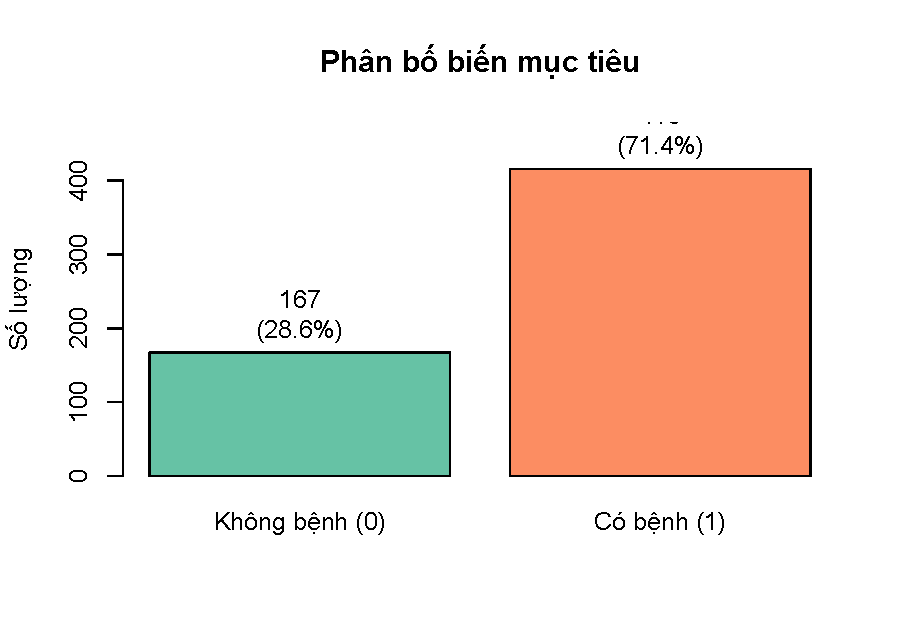
\includegraphics[width=\maxwidth]{figure/tl-target-dist-1} 

}

\caption[Phân bố biến mục tiêu]{Phân bố biến mục tiêu: dữ liệu mất cân bằng lớp theo tỉ lệ xấp xỉ 71/29}\label{fig:target-dist}
\end{figure}

\end{knitrout}

Tỉ lệ 71,4\% / 28,6\% cho thấy dữ liệu mất cân bằng ở mức trung bình. Hệ
quả trực tiếp: \emph{độ chính xác tổng thể} (accuracy) là chỉ số gây hiểu
nhầm --- một mô hình dự đoán tất cả bệnh nhân đều mắc bệnh đã đạt accuracy
$0{,}714$ mà không học được gì. Vì vậy toàn bộ phần đánh giá về sau sẽ báo
cáo recall và precision của \emph{từng lớp} cùng với macro F1, chứ không
dựa vào accuracy.

\subsection{Giới tính và bệnh gan: kiểm định Chi-square}

Trước khi đưa \texttt{Gender} vào mô hình, cần kiểm tra xem biến này có
thực sự liên hệ với biến mục tiêu hay không. Giả thuyết
$H_0$: tỉ lệ mắc bệnh không khác nhau giữa hai giới.

\begin{knitrout}\scriptsize
\definecolor{shadecolor}{rgb}{0.969, 0.969, 0.969}\color{fgcolor}\begin{kframe}
\begin{alltt}
\hldef{contingency} \hlkwb{<-} \hlkwd{table}\hldef{(df}\hlopt{$}\hldef{Gender, df}\hlopt{$}\hldef{target)}
\hlkwd{print}\hldef{(contingency)}
\end{alltt}
\begin{verbatim}
##         
##            0   1
##   Female  50  92
##   Male   117 324
\end{verbatim}
\begin{alltt}
\hldef{chi_res} \hlkwb{<-} \hlkwd{chisq.test}\hldef{(contingency)}
\hlkwd{cat}\hldef{(}\hlsng{"\textbackslash{}nChi-square ="}\hldef{,} \hlkwd{round}\hldef{(chi_res}\hlopt{$}\hldef{statistic,} \hlnum{4}\hldef{),}
    \hlsng{"| p-value ="}\hldef{,} \hlkwd{round}\hldef{(chi_res}\hlopt{$}\hldef{p.value,} \hlnum{4}\hldef{),} \hlsng{"\textbackslash{}n"}\hldef{)}
\end{alltt}
\begin{verbatim}
## 
## Chi-square = 3.5466 | p-value = 0.0597
\end{verbatim}
\begin{alltt}
\hlkwd{cat}\hldef{(}\hlsng{"Bảng tần số kỳ vọng (cần >= 5 để kiểm định hợp lệ):\textbackslash{}n"}\hldef{)}
\end{alltt}
\begin{verbatim}
## Bảng tần số kỳ vọng (cần >= 5 để kiểm định hợp lệ):
\end{verbatim}
\begin{alltt}
\hlkwd{print}\hldef{(}\hlkwd{round}\hldef{(chi_res}\hlopt{$}\hldef{expected,} \hlnum{2}\hldef{))}
\end{alltt}
\begin{verbatim}
##         
##               0      1
##   Female  40.68 101.32
##   Male   126.32 314.68
\end{verbatim}
\end{kframe}
\end{knitrout}

Tần số kỳ vọng ở cả bốn ô đều lớn hơn 5 nên kiểm định hợp lệ. Với
$p = 0{,}0597 > 0{,}05$, ta \emph{không} đủ bằng chứng bác bỏ $H_0$: dữ
liệu chưa cho thấy khác biệt có ý nghĩa thống kê về tỉ lệ mắc bệnh giữa
nam và nữ. Cần lưu ý cách diễn đạt --- ``không bác bỏ được $H_0$'' khác
với ``chứng minh $H_0$ đúng''; giá trị $p$ nằm sát ngưỡng $0{,}05$ nên kết
luận hợp lý là bằng chứng còn yếu chứ không phải liên hệ chắc chắn không
tồn tại.

\subsection{Tương quan giữa các biến}

\begin{knitrout}\tiny
\definecolor{shadecolor}{rgb}{0.969, 0.969, 0.969}\color{fgcolor}\begin{kframe}
\begin{alltt}
\hldef{numeric_cols} \hlkwb{<-} \hlkwd{c}\hldef{(}
  \hlsng{"Age"}\hldef{,} \hlsng{"Total_Bilirubin"}\hldef{,} \hlsng{"Direct_Bilirubin"}\hldef{,} \hlsng{"Alkaline_Phosphotase"}\hldef{,}
  \hlsng{"Alamine_Aminotransferase"}\hldef{,} \hlsng{"Aspartate_Aminotransferase"}\hldef{,}
  \hlsng{"Total_Protiens"}\hldef{,} \hlsng{"Albumin"}\hldef{,} \hlsng{"Albumin_and_Globulin_Ratio"}
\hldef{)}

\hldef{corr_mat} \hlkwb{<-} \hlkwd{cor}\hldef{(df[,} \hlkwd{c}\hldef{(numeric_cols,} \hlsng{"target"}\hldef{)],} \hlkwc{use} \hldef{=} \hlsng{"complete.obs"}\hldef{)}

\hlcom{# Rút gọn tên chỉ để in cho vừa khổ giấy; corr_mat gốc giữ nguyên}
\hldef{corr_disp} \hlkwb{<-} \hlkwd{round}\hldef{(corr_mat,} \hlnum{2}\hldef{)}
\hlkwd{dimnames}\hldef{(corr_disp)} \hlkwb{<-} \hlkwd{list}\hldef{(}\hlkwd{abbreviate}\hldef{(}\hlkwd{rownames}\hldef{(corr_mat),} \hlnum{12}\hldef{),}
                            \hlkwd{abbreviate}\hldef{(}\hlkwd{colnames}\hldef{(corr_mat),} \hlnum{6}\hldef{))}
\hlkwd{print}\hldef{(corr_disp)}
\end{alltt}
\begin{verbatim}
##                Age Ttl_Bl Drct_B Alkl_P Almn_A Aspr_A Ttl_Pr Albumn
## Age           1.00   0.01   0.01   0.08  -0.09  -0.02  -0.19  -0.26
## Total_Bilrbn  0.01   1.00   0.87   0.21   0.21   0.24  -0.01  -0.22
## Direct_Blrbn  0.01   0.87   1.00   0.23   0.23   0.26   0.00  -0.23
## Alkln_Phspht  0.08   0.21   0.23   1.00   0.12   0.17  -0.03  -0.16
## Almn_Amntrns -0.09   0.21   0.23   0.12   1.00   0.79  -0.04  -0.03
## Asprtt_Amntr -0.02   0.24   0.26   0.17   0.79   1.00  -0.03  -0.08
## Total_Protns -0.19  -0.01   0.00  -0.03  -0.04  -0.03   1.00   0.78
## Albumin      -0.26  -0.22  -0.23  -0.16  -0.03  -0.08   0.78   1.00
## Albmn_nd_G_R -0.22  -0.21  -0.20  -0.23   0.00  -0.07   0.23   0.69
## target        0.13   0.22   0.25   0.18   0.16   0.15  -0.03  -0.16
##              A__G_R target
## Age           -0.22   0.13
## Total_Bilrbn  -0.21   0.22
## Direct_Blrbn  -0.20   0.25
## Alkln_Phspht  -0.23   0.18
## Almn_Amntrns   0.00   0.16
## Asprtt_Amntr  -0.07   0.15
## Total_Protns   0.23  -0.03
## Albumin        0.69  -0.16
## Albmn_nd_G_R   1.00  -0.16
## target        -0.16   1.00
\end{verbatim}
\end{kframe}
\end{knitrout}

\begin{knitrout}\scriptsize
\definecolor{shadecolor}{rgb}{0.969, 0.969, 0.969}\color{fgcolor}\begin{kframe}
\begin{alltt}
\hlkwd{par}\hldef{(}\hlkwc{mar} \hldef{=} \hlkwd{c}\hldef{(}\hlnum{9}\hldef{,} \hlnum{9}\hldef{,} \hlnum{3}\hldef{,} \hlnum{2}\hldef{))}
\hlkwd{image}\hldef{(}\hlkwd{seq_len}\hldef{(}\hlkwd{ncol}\hldef{(corr_mat)),} \hlkwd{seq_len}\hldef{(}\hlkwd{nrow}\hldef{(corr_mat)),}
      \hlkwd{t}\hldef{(corr_mat[}\hlkwd{nrow}\hldef{(corr_mat)}\hlopt{:}\hlnum{1}\hldef{, ]),}
      \hlkwc{col} \hldef{=} \hlkwd{colorRampPalette}\hldef{(}\hlkwd{c}\hldef{(}\hlsng{"#3288bd"}\hldef{,} \hlsng{"white"}\hldef{,} \hlsng{"#d53e4f"}\hldef{))(}\hlnum{64}\hldef{),}
      \hlkwc{zlim} \hldef{=} \hlkwd{c}\hldef{(}\hlopt{-}\hlnum{1}\hldef{,} \hlnum{1}\hldef{),} \hlkwc{axes} \hldef{=} \hlnum{FALSE}\hldef{,} \hlkwc{xlab} \hldef{=} \hlsng{""}\hldef{,} \hlkwc{ylab} \hldef{=} \hlsng{""}\hldef{,}
      \hlkwc{main} \hldef{=} \hlsng{"Ma trận tương quan"}\hldef{)}
\hlkwd{axis}\hldef{(}\hlnum{1}\hldef{,} \hlkwd{seq_len}\hldef{(}\hlkwd{ncol}\hldef{(corr_mat)),} \hlkwd{colnames}\hldef{(corr_mat),} \hlkwc{las} \hldef{=} \hlnum{2}\hldef{,} \hlkwc{cex.axis} \hldef{=} \hlnum{0.7}\hldef{)}
\hlkwd{axis}\hldef{(}\hlnum{2}\hldef{,} \hlkwd{seq_len}\hldef{(}\hlkwd{nrow}\hldef{(corr_mat)),} \hlkwd{rev}\hldef{(}\hlkwd{rownames}\hldef{(corr_mat)),} \hlkwc{las} \hldef{=} \hlnum{2}\hldef{,}
     \hlkwc{cex.axis} \hldef{=} \hlnum{0.7}\hldef{)}
\end{alltt}
\end{kframe}\begin{figure}

{\centering 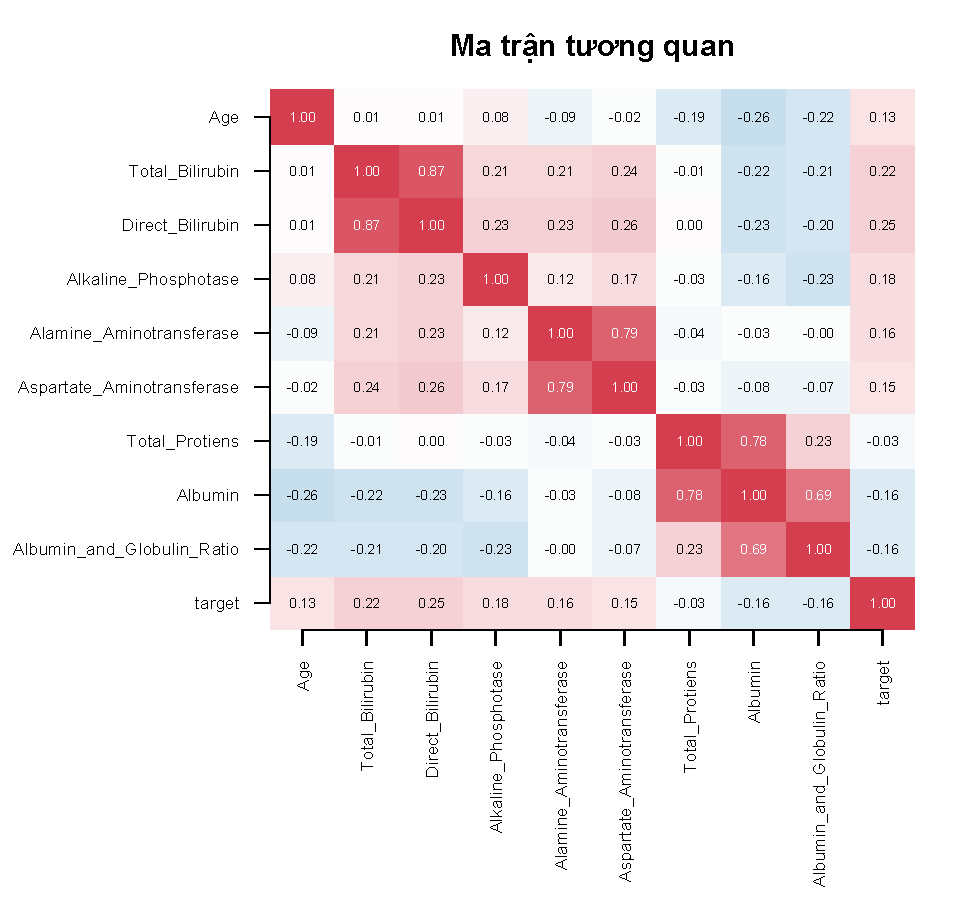
\includegraphics[width=\maxwidth]{figure/tl-corr-heatmap-1} 

}

\caption[Ma trận tương quan giữa các biến sinh hoá và biến mục tiêu]{Ma trận tương quan giữa các biến sinh hoá và biến mục tiêu}\label{fig:corr-heatmap}
\end{figure}

\begin{kframe}\begin{alltt}
\hlkwd{par}\hldef{(}\hlkwc{mar} \hldef{=} \hlkwd{c}\hldef{(}\hlnum{5}\hldef{,} \hlnum{4}\hldef{,} \hlnum{4}\hldef{,} \hlnum{2}\hldef{)} \hlopt{+} \hlnum{0.1}\hldef{)}
\end{alltt}
\end{kframe}
\end{knitrout}

Ba cặp biến có tương quan rất cao nổi lên rõ rệt:
\texttt{Total\_Bilirubin} với \texttt{Direct\_Bilirubin} ($r = 0{,}87$),
\texttt{Alamine\_Aminotransferase} với
\texttt{Aspartate\_Aminotransferase} ($r = 0{,}79$), và
\texttt{Total\_Protiens} với \texttt{Albumin} ($r = 0{,}78$). Điều này dễ
hiểu về mặt sinh hoá --- bilirubin trực tiếp là một thành phần của
bilirubin toàn phần, còn albumin là thành phần chính của protein toàn
phần --- nhưng lại là vấn đề đối với hồi quy logistic, vì các biến gần
như trùng thông tin làm ma trận thiết kế gần suy biến và hệ số ước lượng
mất ổn định. Đồng thời, tương quan với \texttt{target} của mọi biến đều
yếu (giá trị lớn nhất là $0{,}25$), báo trước rằng không có biến đơn lẻ
nào tách được hai nhóm một cách rõ ràng.

\subsection{Đa cộng tuyến: hệ số VIF}

Tương quan từng cặp chỉ phát hiện được quan hệ hai biến. Hệ số phóng đại
phương sai (Variance Inflation Factor) đo mức độ một biến bị giải thích
bởi \emph{toàn bộ} các biến còn lại:
\[
  \mathrm{VIF}_j = \frac{1}{1 - R_j^2},
\]
với $R_j^2$ là hệ số xác định của hồi quy biến $j$ lên tất cả các biến
khác. Hàm dưới đây tự cài đặt công thức đó bằng \texttt{lm()}, không cần
gói \texttt{car}.

\begin{knitrout}\scriptsize
\definecolor{shadecolor}{rgb}{0.969, 0.969, 0.969}\color{fgcolor}\begin{kframe}
\begin{alltt}
\hldef{compute_vif} \hlkwb{<-} \hlkwa{function}\hldef{(}\hlkwc{data}\hldef{) \{}
  \hldef{vars} \hlkwb{<-} \hlkwd{colnames}\hldef{(data)}
  \hlkwd{sapply}\hldef{(vars,} \hlkwa{function}\hldef{(}\hlkwc{v}\hldef{) \{}
    \hldef{others} \hlkwb{<-} \hlkwd{setdiff}\hldef{(vars, v)}
    \hldef{fml} \hlkwb{<-} \hlkwd{as.formula}\hldef{(}\hlkwd{paste}\hldef{(v,} \hlsng{"~"}\hldef{,} \hlkwd{paste}\hldef{(others,} \hlkwc{collapse} \hldef{=} \hlsng{" + "}\hldef{)))}
    \hldef{r2} \hlkwb{<-} \hlkwd{summary}\hldef{(}\hlkwd{lm}\hldef{(fml,} \hlkwc{data} \hldef{= data))}\hlopt{$}\hldef{r.squared}
    \hlnum{1} \hlopt{/} \hldef{(}\hlnum{1} \hlopt{-} \hldef{r2)}
  \hldef{\})}
\hldef{\}}

\hldef{X_vif} \hlkwb{<-} \hldef{df[,} \hlkwd{c}\hldef{(numeric_cols,} \hlsng{"Gender"}\hldef{)]}
\hldef{X_vif}\hlopt{$}\hldef{Gender} \hlkwb{<-} \hlkwd{ifelse}\hldef{(X_vif}\hlopt{$}\hldef{Gender} \hlopt{==} \hlsng{"Male"}\hldef{,} \hlnum{1}\hldef{,} \hlnum{0}\hldef{)}
\hldef{X_vif}\hlopt{$}\hldef{Albumin_and_Globulin_Ratio[}\hlkwd{is.na}\hldef{(X_vif}\hlopt{$}\hldef{Albumin_and_Globulin_Ratio)]} \hlkwb{<-}
  \hlkwd{median}\hldef{(X_vif}\hlopt{$}\hldef{Albumin_and_Globulin_Ratio,} \hlkwc{na.rm} \hldef{=} \hlnum{TRUE}\hldef{)}

\hldef{vif_raw} \hlkwb{<-} \hlkwd{compute_vif}\hldef{(X_vif)}
\hlkwd{print}\hldef{(}\hlkwd{round}\hldef{(}\hlkwd{sort}\hldef{(vif_raw,} \hlkwc{decreasing} \hldef{=} \hlnum{TRUE}\hldef{),} \hlnum{3}\hldef{))}
\end{alltt}
\begin{verbatim}
##                    Albumin             Total_Protiens 
##                     10.124                      5.549 
##           Direct_Bilirubin            Total_Bilirubin 
##                      4.525                      4.277 
## Albumin_and_Globulin_Ratio   Alamine_Aminotransferase 
##                      3.683                      2.820 
## Aspartate_Aminotransferase       Alkaline_Phosphotase 
##                      2.811                      1.122 
##                        Age                     Gender 
##                      1.099                      1.034
\end{verbatim}
\end{kframe}
\end{knitrout}

Theo quy ước thường dùng, $\mathrm{VIF} > 5$ là đáng lo và
$\mathrm{VIF} > 10$ là nghiêm trọng. \texttt{Albumin} vượt ngưỡng 10 và
\texttt{Total\_Protiens} vượt ngưỡng 5, đúng như cặp tương quan $0{,}78$
đã gợi ý.

\subsection{Phân bố các biến sinh hoá theo nhóm}

\begin{knitrout}\scriptsize
\definecolor{shadecolor}{rgb}{0.969, 0.969, 0.969}\color{fgcolor}\begin{kframe}
\begin{alltt}
\hlkwd{par}\hldef{(}\hlkwc{mfrow} \hldef{=} \hlkwd{c}\hldef{(}\hlnum{3}\hldef{,} \hlnum{3}\hldef{),} \hlkwc{mar} \hldef{=} \hlkwd{c}\hldef{(}\hlnum{4}\hldef{,} \hlnum{4}\hldef{,} \hlnum{3}\hldef{,} \hlnum{1}\hldef{))}
\hlkwa{for} \hldef{(col} \hlkwa{in} \hldef{numeric_cols) \{}
  \hlkwd{boxplot}\hldef{(df[[col]]} \hlopt{~} \hldef{df}\hlopt{$}\hldef{target,} \hlkwc{col} \hldef{=} \hlkwd{c}\hldef{(}\hlsng{"#66c2a5"}\hldef{,} \hlsng{"#fc8d62"}\hldef{),}
          \hlkwc{main} \hldef{= col,} \hlkwc{xlab} \hldef{=} \hlsng{"target"}\hldef{,} \hlkwc{ylab} \hldef{=} \hlsng{""}\hldef{)}
\hldef{\}}
\end{alltt}
\end{kframe}\begin{figure}

{\centering 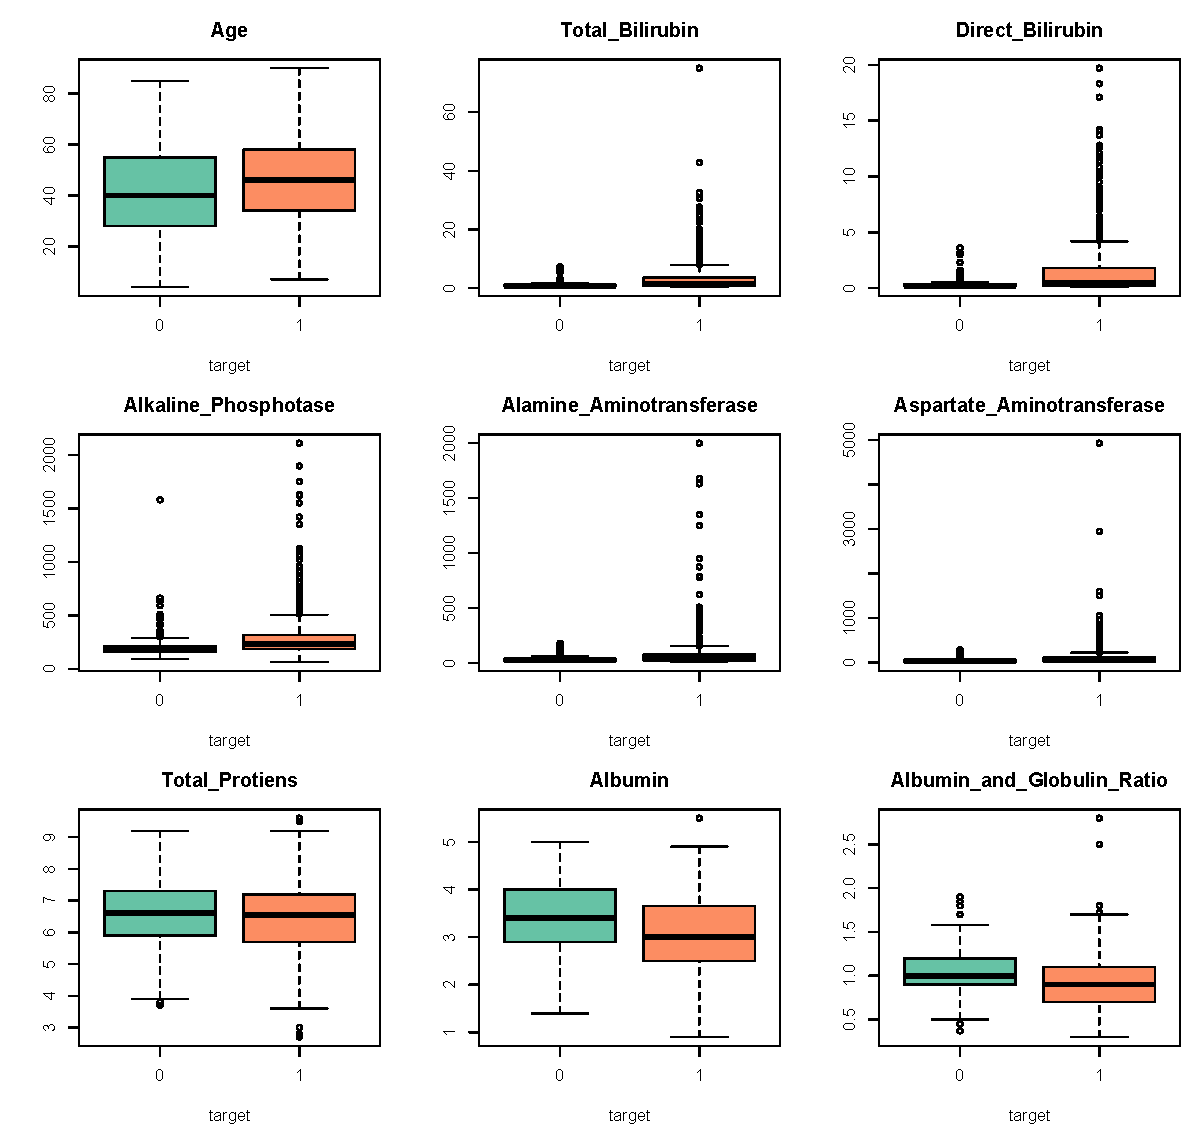
\includegraphics[width=\maxwidth]{figure/tl-boxplot-raw-1} 

}

\caption[Phân bố 9 biến số theo nhóm bệnh, thang đo gốc]{Phân bố 9 biến số theo nhóm bệnh, thang đo gốc. Các men gan lệch phải rất nặng}\label{fig:boxplot-raw}
\end{figure}

\begin{kframe}\begin{alltt}
\hlkwd{par}\hldef{(}\hlkwc{mfrow} \hldef{=} \hlkwd{c}\hldef{(}\hlnum{1}\hldef{,} \hlnum{1}\hldef{),} \hlkwc{mar} \hldef{=} \hlkwd{c}\hldef{(}\hlnum{5}\hldef{,} \hlnum{4}\hldef{,} \hlnum{4}\hldef{,} \hlnum{2}\hldef{)} \hlopt{+} \hlnum{0.1}\hldef{)}
\end{alltt}
\end{kframe}
\end{knitrout}

Hình~\ref{fig:boxplot-raw} cho thấy năm biến --- hai loại bilirubin và ba
men gan --- lệch phải cực nặng: hộp bị nén sát trục còn các điểm ngoại lai
kéo dài lên trên. Đây là dạng phân bố điển hình của chỉ số men gan.

\subsection{Biến đổi log1p cho các biến lệch phải}

Cách xử lý ngoại lai quen thuộc là winsorization (kẹp giá trị ở phân vị
1\% và 99\%). Ở đây cách đó \emph{không} phù hợp: các giá trị cực đại là
tín hiệu lâm sàng thật --- AST khoảng 5000 U/L tương ứng với suy gan cấp
--- và chúng tập trung ở nhóm bệnh, nên kẹp chúng lại chính là xoá đi
thông tin phân biệt hai lớp. Phép biến đổi $\log(1+x)$ là lựa chọn thích
hợp hơn: nó nén đuôi phân phối mà vẫn \emph{bảo toàn thứ hạng} của các
quan sát, do là hàm đơn điệu tăng.

\begin{knitrout}\scriptsize
\definecolor{shadecolor}{rgb}{0.969, 0.969, 0.969}\color{fgcolor}\begin{kframe}
\begin{alltt}
\hldef{skewed_cols} \hlkwb{<-} \hlkwd{c}\hldef{(}\hlsng{"Total_Bilirubin"}\hldef{,} \hlsng{"Direct_Bilirubin"}\hldef{,}
                 \hlsng{"Alkaline_Phosphotase"}\hldef{,} \hlsng{"Alamine_Aminotransferase"}\hldef{,}
                 \hlsng{"Aspartate_Aminotransferase"}\hldef{)}

\hldef{df_raw} \hlkwb{<-} \hldef{df}                       \hlcom{# giữ bản gốc để tra thang đo lâm sàng}
\hlkwa{for} \hldef{(col} \hlkwa{in} \hldef{skewed_cols) df[[col]]} \hlkwb{<-} \hlkwd{log1p}\hldef{(df[[col]])}

\hlcom{# Hệ số bất đối xứng, tự tính vì base R không có hàm skewness}
\hldef{skewness} \hlkwb{<-} \hlkwa{function}\hldef{(}\hlkwc{x}\hldef{) \{}
  \hldef{x} \hlkwb{<-} \hldef{x[}\hlopt{!}\hlkwd{is.na}\hldef{(x)]}
  \hlkwd{mean}\hldef{((x} \hlopt{-} \hlkwd{mean}\hldef{(x))}\hlopt{^}\hlnum{3}\hldef{)} \hlopt{/} \hldef{(}\hlkwd{mean}\hldef{((x} \hlopt{-} \hlkwd{mean}\hldef{(x))}\hlopt{^}\hlnum{2}\hldef{))}\hlopt{^}\hlnum{1.5}
\hldef{\}}

\hlkwd{print}\hldef{(}\hlkwd{round}\hldef{(}\hlkwd{data.frame}\hldef{(}
  \hlkwc{goc}       \hldef{=} \hlkwd{sapply}\hldef{(df_raw[skewed_cols], skewness),}
  \hlkwc{sau_log1p} \hldef{=} \hlkwd{sapply}\hldef{(df[skewed_cols], skewness)}
\hldef{),} \hlnum{2}\hldef{))}
\end{alltt}
\begin{verbatim}
##                              goc sau_log1p
## Total_Bilirubin             4.89      1.72
## Direct_Bilirubin            3.20      1.68
## Alkaline_Phosphotase        3.76      1.33
## Alamine_Aminotransferase    6.53      1.47
## Aspartate_Aminotransferase 10.52      1.23
\end{verbatim}
\end{kframe}
\end{knitrout}

Hiệu quả rất rõ: \texttt{Aspartate\_Aminotransferase} giảm hệ số bất đối
xứng từ $10{,}52$ xuống $1{,}23$, \texttt{Alamine\_Aminotransferase} từ
$6{,}53$ xuống $1{,}47$. Cả năm biến đều về mức bất đối xứng nhẹ.

\begin{knitrout}\scriptsize
\definecolor{shadecolor}{rgb}{0.969, 0.969, 0.969}\color{fgcolor}\begin{kframe}
\begin{alltt}
\hlkwd{par}\hldef{(}\hlkwc{mfrow} \hldef{=} \hlkwd{c}\hldef{(}\hlnum{3}\hldef{,} \hlnum{3}\hldef{),} \hlkwc{mar} \hldef{=} \hlkwd{c}\hldef{(}\hlnum{4}\hldef{,} \hlnum{4}\hldef{,} \hlnum{3}\hldef{,} \hlnum{1}\hldef{))}
\hlkwa{for} \hldef{(col} \hlkwa{in} \hldef{numeric_cols) \{}
  \hlkwd{boxplot}\hldef{(df[[col]]} \hlopt{~} \hldef{df}\hlopt{$}\hldef{target,} \hlkwc{col} \hldef{=} \hlkwd{c}\hldef{(}\hlsng{"#66c2a5"}\hldef{,} \hlsng{"#fc8d62"}\hldef{),}
          \hlkwc{main} \hldef{=} \hlkwa{if} \hldef{(col} \hlopt{%in%} \hldef{skewed_cols)} \hlkwd{paste0}\hldef{(}\hlsng{"log1p("}\hldef{, col,} \hlsng{")"}\hldef{)} \hlkwa{else} \hldef{col,}
          \hlkwc{xlab} \hldef{=} \hlsng{"target"}\hldef{,} \hlkwc{ylab} \hldef{=} \hlsng{""}\hldef{)}
\hldef{\}}
\end{alltt}
\end{kframe}\begin{figure}

{\centering 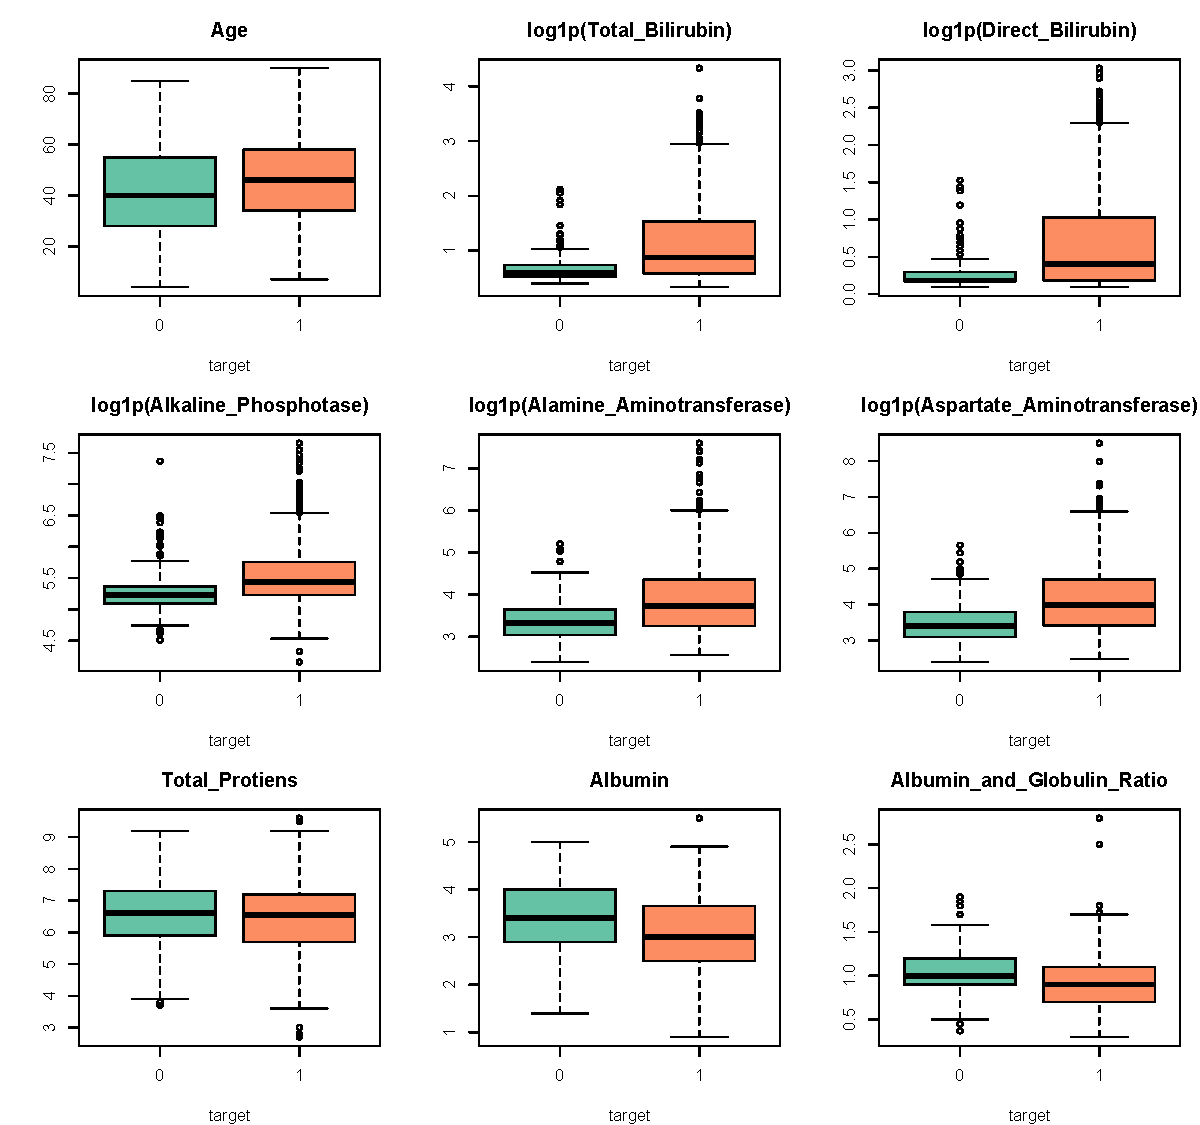
\includegraphics[width=\maxwidth]{figure/tl-boxplot-log-1} 

}

\caption[Phân bố sau khi biến đổi log1p]{Phân bố sau khi biến đổi log1p. Khác biệt giữa hai nhóm trở nên nhìn được}\label{fig:boxplot-log}
\end{figure}

\begin{kframe}\begin{alltt}
\hlkwd{par}\hldef{(}\hlkwc{mfrow} \hldef{=} \hlkwd{c}\hldef{(}\hlnum{1}\hldef{,} \hlnum{1}\hldef{),} \hlkwc{mar} \hldef{=} \hlkwd{c}\hldef{(}\hlnum{5}\hldef{,} \hlnum{4}\hldef{,} \hlnum{4}\hldef{,} \hlnum{2}\hldef{)} \hlopt{+} \hlnum{0.1}\hldef{)}
\end{alltt}
\end{kframe}
\end{knitrout}

\subsection{VIF tính lại trên thang log}

Một điểm dễ bị bỏ qua: hệ số tương quan Pearson và VIF \emph{không} bất
biến với phép biến đổi log (khác với các kiểm định dựa trên thứ hạng). Ma
trận thiết kế mà mô hình thực sự sử dụng là ma trận trên thang log, nên
VIF phải được tính lại trên đúng thang đó.

\begin{knitrout}\scriptsize
\definecolor{shadecolor}{rgb}{0.969, 0.969, 0.969}\color{fgcolor}\begin{kframe}
\begin{alltt}
\hldef{X_vif_log} \hlkwb{<-} \hldef{X_vif}
\hlkwa{for} \hldef{(col} \hlkwa{in} \hldef{skewed_cols) X_vif_log[[col]]} \hlkwb{<-} \hlkwd{log1p}\hldef{(df_raw[[col]])}
\hldef{vif_log} \hlkwb{<-} \hlkwd{compute_vif}\hldef{(X_vif_log)}

\hlkwd{print}\hldef{(}\hlkwd{round}\hldef{(}\hlkwd{data.frame}\hldef{(}
  \hlkwc{VIF_goc}    \hldef{= vif_raw,}
  \hlkwc{VIF_log}    \hldef{= vif_log[}\hlkwd{names}\hldef{(vif_raw)],}
  \hlkwc{chenh_lech} \hldef{= vif_log[}\hlkwd{names}\hldef{(vif_raw)]} \hlopt{-} \hldef{vif_raw}
\hldef{)[}\hlkwd{order}\hldef{(}\hlopt{-}\hldef{vif_log[}\hlkwd{names}\hldef{(vif_raw)]), ],} \hlnum{2}\hldef{))}
\end{alltt}
\begin{verbatim}
##                            VIF_goc VIF_log chenh_lech
## Total_Bilirubin               4.28   20.72      16.44
## Direct_Bilirubin              4.53   20.55      16.03
## Albumin                      10.12   10.62       0.49
## Total_Protiens                5.55    5.65       0.10
## Aspartate_Aminotransferase    2.81    4.18       1.37
## Alamine_Aminotransferase      2.82    3.94       1.12
## Albumin_and_Globulin_Ratio    3.68    3.75       0.07
## Alkaline_Phosphotase          1.12    1.28       0.16
## Age                           1.10    1.10       0.00
## Gender                        1.03    1.06       0.03
\end{verbatim}
\end{kframe}
\end{knitrout}

Kết quả thay đổi hẳn bức tranh. Trên thang gốc, hai biến bilirubin có VIF
chỉ khoảng $4{,}3$--$4{,}5$; trên thang log chúng vọt lên trên $20$ ---
mức nghiêm trọng. Nguyên nhân là quan hệ giữa hai biến này vốn có dạng
nhân tính, và phép lấy log đã biến nó thành quan hệ tuyến tính gần như
hoàn hảo. Nếu chỉ nhìn VIF trên thang gốc, ta sẽ kết luận sai rằng cặp
bilirubin không có vấn đề. Đây là căn cứ trực tiếp để loại
\texttt{Direct\_Bilirubin} khỏi mô hình.

\subsection{Thống kê mô tả theo nhóm}

Bảng dưới đây được tính trên \texttt{df\_raw} --- thang đo gốc --- để các
con số còn giữ nguyên đơn vị lâm sàng và có thể đối chiếu với khoảng tham
chiếu xét nghiệm.

\begin{knitrout}\tiny
\definecolor{shadecolor}{rgb}{0.969, 0.969, 0.969}\color{fgcolor}\begin{kframe}
\begin{alltt}
\hlkwa{for} \hldef{(col} \hlkwa{in} \hldef{numeric_cols) \{}
  \hldef{s} \hlkwb{<-} \hlkwd{tapply}\hldef{(df_raw[[col]], df_raw}\hlopt{$}\hldef{target,} \hlkwa{function}\hldef{(}\hlkwc{x}\hldef{) \{}
    \hldef{x} \hlkwb{<-} \hldef{x[}\hlopt{!}\hlkwd{is.na}\hldef{(x)]}
    \hlkwd{c}\hldef{(}\hlkwc{min} \hldef{=} \hlkwd{min}\hldef{(x),} \hlkwc{max} \hldef{=} \hlkwd{max}\hldef{(x),} \hlkwc{mean} \hldef{=} \hlkwd{mean}\hldef{(x),}
      \hlkwc{median} \hldef{=} \hlkwd{median}\hldef{(x),} \hlkwc{sd} \hldef{=} \hlkwd{sd}\hldef{(x))}
  \hldef{\})}
  \hlkwd{cat}\hldef{(}\hlsng{"\textbackslash{}n"}\hldef{, col,} \hlsng{"\textbackslash{}n"}\hldef{)}
  \hlkwd{print}\hldef{(}\hlkwd{round}\hldef{(}\hlkwd{do.call}\hldef{(rbind, s),} \hlnum{2}\hldef{))}
\hldef{\}}
\end{alltt}
\begin{verbatim}
## 
##  Age 
##   min max  mean median    sd
## 0   4  85 41.24     40 17.00
## 1   7  90 46.15     46 15.65
## 
##  Total_Bilirubin 
##   min  max mean median   sd
## 0 0.5  7.3 1.14    0.8 1.00
## 1 0.4 75.0 4.16    1.4 7.14
## 
##  Direct_Bilirubin 
##   min  max mean median   sd
## 0 0.1  3.6 0.40    0.2 0.52
## 1 0.1 19.7 1.92    0.5 3.21
## 
##  Alkaline_Phosphotase 
##   min  max   mean median     sd
## 0  90 1580 219.75    186 140.99
## 1  63 2110 319.01    229 268.31
## 
##  Alamine_Aminotransferase 
##   min  max  mean median     sd
## 0  10  181 33.65     27  25.06
## 1  12 2000 99.61     41 212.77
## 
##  Aspartate_Aminotransferase 
##   min  max   mean median     sd
## 0  10  285  40.69   29.0  36.41
## 1  11 4929 137.70   52.5 337.39
## 
##  Total_Protiens 
##   min max mean median   sd
## 0 3.7 9.2 6.54   6.60 1.06
## 1 2.7 9.6 6.46   6.55 1.09
## 
##  Albumin 
##   min max mean median   sd
## 0 1.4 5.0 3.34    3.4 0.78
## 1 0.9 5.5 3.06    3.0 0.79
## 
##  Albumin_and_Globulin_Ratio 
##    min max mean median   sd
## 0 0.37 1.9 1.03    1.0 0.29
## 1 0.30 2.8 0.91    0.9 0.33
\end{verbatim}
\end{kframe}
\end{knitrout}

Chênh lệch giữa trung bình và trung vị ở nhóm bệnh rất lớn --- chẳng hạn
\texttt{Aspartate\_Aminotransferase} có trung bình $137{,}7$ nhưng trung
vị chỉ $52{,}5$ --- một lần nữa khẳng định phân phối lệch nặng và củng cố
lựa chọn dùng kiểm định phi tham số ở bước tiếp theo.

\subsection{Chọn biến: Mann-Whitney U và hiệu chỉnh FDR}

Vì phần lớn biến lệch phải nặng, kiểm định $t$ (giả định phân phối chuẩn)
không phù hợp. Ta dùng kiểm định Mann-Whitney U, dựa trên thứ hạng nên
không đòi hỏi giả định về dạng phân phối --- và cũng vì thế, giá trị $p$
của nó \emph{không đổi} sau phép biến đổi log1p ở trên.

Kích thước ảnh hưởng đi kèm là hệ số tương quan \emph{rank-biserial}, nằm
trong $[-1, 1]$:
\[
  r_{rb} = 1 - \frac{2U}{n_0 n_1}.
\]
Riêng biến \texttt{Gender} là biến phân loại nên dùng kết quả Chi-square ở
trên với kích thước ảnh hưởng Cramér's V.

Một vấn đề nữa cần xử lý: ta chạy 10 kiểm định cùng lúc ở mức $\alpha =
0{,}05$. Xác suất có ít nhất một kết quả dương tính giả khi đó không còn
là 5\% nữa. Thủ tục Benjamini--Hochberg hiệu chỉnh giá trị $p$ để kiểm
soát \emph{tỉ lệ phát hiện sai} (False Discovery Rate).

\begin{knitrout}\scriptsize
\definecolor{shadecolor}{rgb}{0.969, 0.969, 0.969}\color{fgcolor}\begin{kframe}
\begin{alltt}
\hldef{fs} \hlkwb{<-} \hlkwd{data.frame}\hldef{(}\hlkwc{feature} \hldef{=} \hlkwd{character}\hldef{(),} \hlkwc{p_value} \hldef{=} \hlkwd{numeric}\hldef{(),}
                 \hlkwc{effect_size} \hldef{=} \hlkwd{numeric}\hldef{(),} \hlkwc{stringsAsFactors} \hldef{=} \hlnum{FALSE}\hldef{)}

\hlkwa{for} \hldef{(col} \hlkwa{in} \hldef{numeric_cols) \{}
  \hldef{g0} \hlkwb{<-} \hldef{df[[col]][df}\hlopt{$}\hldef{target} \hlopt{==} \hlnum{0}\hldef{]}
  \hldef{g1} \hlkwb{<-} \hldef{df[[col]][df}\hlopt{$}\hldef{target} \hlopt{==} \hlnum{1}\hldef{]}
  \hldef{w} \hlkwb{<-} \hlkwd{wilcox.test}\hldef{(g0, g1,} \hlkwc{exact} \hldef{=} \hlnum{FALSE}\hldef{)}
  \hldef{n0} \hlkwb{<-} \hlkwd{sum}\hldef{(}\hlopt{!}\hlkwd{is.na}\hldef{(g0)); n1} \hlkwb{<-} \hlkwd{sum}\hldef{(}\hlopt{!}\hlkwd{is.na}\hldef{(g1))}
  \hldef{rb} \hlkwb{<-} \hlnum{1} \hlopt{-} \hlnum{2} \hlopt{*} \hldef{w}\hlopt{$}\hldef{statistic} \hlopt{/} \hldef{(n0} \hlopt{*} \hldef{n1)}     \hlcom{# rank-biserial correlation}
  \hldef{fs} \hlkwb{<-} \hlkwd{rbind}\hldef{(fs,} \hlkwd{data.frame}\hldef{(}\hlkwc{feature} \hldef{= col,} \hlkwc{p_value} \hldef{= w}\hlopt{$}\hldef{p.value,}
                             \hlkwc{effect_size} \hldef{=} \hlkwd{as.numeric}\hldef{(rb)))}
\hldef{\}}

\hlcom{# Gender: dùng Cramer's V làm kích thước ảnh hưởng}
\hldef{n_total} \hlkwb{<-} \hlkwd{sum}\hldef{(contingency)}
\hldef{cramers_v} \hlkwb{<-} \hlkwd{sqrt}\hldef{(chi_res}\hlopt{$}\hldef{statistic} \hlopt{/}
                    \hldef{(n_total} \hlopt{*} \hldef{(}\hlkwd{min}\hldef{(}\hlkwd{dim}\hldef{(contingency))} \hlopt{-} \hlnum{1}\hldef{)))}
\hldef{fs} \hlkwb{<-} \hlkwd{rbind}\hldef{(fs,} \hlkwd{data.frame}\hldef{(}\hlkwc{feature} \hldef{=} \hlsng{"Gender"}\hldef{,} \hlkwc{p_value} \hldef{= chi_res}\hlopt{$}\hldef{p.value,}
                           \hlkwc{effect_size} \hldef{=} \hlkwd{as.numeric}\hldef{(cramers_v)))}

\hldef{fs}\hlopt{$}\hldef{p_fdr} \hlkwb{<-} \hlkwd{p.adjust}\hldef{(fs}\hlopt{$}\hldef{p_value,} \hlkwc{method} \hldef{=} \hlsng{"BH"}\hldef{)}   \hlcom{# Benjamini-Hochberg}
\hldef{fs}\hlopt{$}\hldef{significant} \hlkwb{<-} \hldef{fs}\hlopt{$}\hldef{p_fdr} \hlopt{<} \hlnum{0.05}
\hldef{fs} \hlkwb{<-} \hldef{fs[}\hlkwd{order}\hldef{(fs}\hlopt{$}\hldef{p_value), ]}

\hldef{fs_disp} \hlkwb{<-} \hldef{fs}
\hldef{fs_disp}\hlopt{$}\hldef{p_value} \hlkwb{<-} \hlkwd{signif}\hldef{(fs_disp}\hlopt{$}\hldef{p_value,} \hlnum{3}\hldef{)}
\hldef{fs_disp}\hlopt{$}\hldef{effect_size} \hlkwb{<-} \hlkwd{round}\hldef{(fs_disp}\hlopt{$}\hldef{effect_size,} \hlnum{3}\hldef{)}
\hldef{fs_disp}\hlopt{$}\hldef{p_fdr} \hlkwb{<-} \hlkwd{signif}\hldef{(fs_disp}\hlopt{$}\hldef{p_fdr,} \hlnum{3}\hldef{)}
\hlkwd{print}\hldef{(fs_disp,} \hlkwc{row.names} \hldef{=} \hlnum{FALSE}\hldef{)}
\end{alltt}
\begin{verbatim}
##                     feature  p_value effect_size    p_fdr significant
##  Aspartate_Aminotransferase 9.21e-14       0.394 9.21e-13        TRUE
##             Total_Bilirubin 2.29e-13       0.387 1.14e-12        TRUE
##            Direct_Bilirubin 7.43e-13       0.372 2.48e-12        TRUE
##    Alamine_Aminotransferase 2.33e-12       0.371 5.83e-12        TRUE
##        Alkaline_Phosphotase 4.35e-11       0.349 8.69e-11        TRUE
##  Albumin_and_Globulin_Ratio 5.81e-06      -0.240 9.69e-06        TRUE
##                     Albumin 5.57e-05      -0.213 7.95e-05        TRUE
##                         Age 1.77e-03       0.165 2.22e-03        TRUE
##                      Gender 5.97e-02       0.078 6.63e-02       FALSE
##              Total_Protiens 4.37e-01      -0.041 4.37e-01       FALSE
\end{verbatim}
\end{kframe}
\end{knitrout}

Tám trên mười biến có ý nghĩa thống kê sau hiệu chỉnh FDR. Hai biến bị
loại là \texttt{Gender} ($p_{FDR} = 0{,}066$) và \texttt{Total\_Protiens}
($p_{FDR} = 0{,}437$). Nhóm men gan và bilirubin có kích thước ảnh hưởng
lớn nhất (khoảng $0{,}35$--$0{,}39$), trong khi \texttt{Age} tuy có ý
nghĩa thống kê nhưng kích thước ảnh hưởng chỉ $0{,}17$ --- một lời nhắc
rằng ý nghĩa thống kê và ý nghĩa thực tiễn là hai chuyện khác nhau.

\section{Thiết kế quy trình mô hình hoá}

\subsection{Tập biến đưa vào mô hình}

Từ 10 biến ban đầu, ba biến bị loại với lý do khác nhau:
\texttt{Direct\_Bilirubin} vì trùng thông tin với \texttt{Total\_Bilirubin}
($r = 0{,}87$, VIF trên thang log khoảng 20); \texttt{Gender} và
\texttt{Total\_Protiens} vì không đạt ngưỡng FDR.

\begin{knitrout}\scriptsize
\definecolor{shadecolor}{rgb}{0.969, 0.969, 0.969}\color{fgcolor}\begin{kframe}
\begin{alltt}
\hldef{model_cols} \hlkwb{<-} \hlkwd{c}\hldef{(}\hlsng{"Age"}\hldef{,} \hlsng{"Total_Bilirubin"}\hldef{,} \hlsng{"Alkaline_Phosphotase"}\hldef{,}
                \hlsng{"Alamine_Aminotransferase"}\hldef{,} \hlsng{"Aspartate_Aminotransferase"}\hldef{,}
                \hlsng{"Albumin"}\hldef{,} \hlsng{"Albumin_and_Globulin_Ratio"}\hldef{)}

\hldef{X_all} \hlkwb{<-} \hlkwd{as.matrix}\hldef{(df[, model_cols])}
\hldef{y_all} \hlkwb{<-} \hldef{df}\hlopt{$}\hldef{target}
\end{alltt}
\end{kframe}
\end{knitrout}

Cần thừa nhận rằng đa cộng tuyến chưa được loại bỏ hoàn toàn:
\texttt{Albumin} và \texttt{Albumin\_and\_Globulin\_Ratio} vẫn liên quan
chặt về mặt định nghĩa, và cặp men gan ALT/AST vẫn còn tương quan
$0{,}79$. Đây là một lý do nữa để dùng hồi quy có điều chuẩn ridge ở
Mục~\ref{sec:ridge} --- ridge xử lý được đa cộng tuyến còn lại bằng cách
co các hệ số tương quan về phía nhau thay vì để chúng dao động ngược
chiều.

\subsection{Chia phân tầng và gán fold}

Cả hai hàm dưới đây đều xáo trộn \emph{trong nội bộ từng lớp} rồi mới
chia, nhờ vậy tỉ lệ 71/29 được giữ nguyên ở mọi tập con.

\begin{knitrout}\scriptsize
\definecolor{shadecolor}{rgb}{0.969, 0.969, 0.969}\color{fgcolor}\begin{kframe}
\begin{alltt}
\hldef{stratified_split} \hlkwb{<-} \hlkwa{function}\hldef{(}\hlkwc{y}\hldef{,} \hlkwc{test_frac} \hldef{=} \hlnum{0.2}\hldef{,} \hlkwc{seed} \hldef{=} \hlnum{42}\hldef{) \{}
  \hlkwd{set.seed}\hldef{(seed)}
  \hldef{test_idx} \hlkwb{<-} \hlkwd{integer}\hldef{(}\hlnum{0}\hldef{)}
  \hlkwa{for} \hldef{(cls} \hlkwa{in} \hlkwd{sort}\hldef{(}\hlkwd{unique}\hldef{(y))) \{}
    \hldef{idx} \hlkwb{<-} \hlkwd{which}\hldef{(y} \hlopt{==} \hldef{cls)}
    \hldef{test_idx} \hlkwb{<-} \hlkwd{c}\hldef{(test_idx,} \hlkwd{sample}\hldef{(idx,} \hlkwd{round}\hldef{(}\hlkwd{length}\hldef{(idx)} \hlopt{*} \hldef{test_frac)))}
  \hldef{\}}
  \hlkwd{list}\hldef{(}\hlkwc{train} \hldef{=} \hlkwd{setdiff}\hldef{(}\hlkwd{seq_along}\hldef{(y), test_idx),} \hlkwc{test} \hldef{=} \hlkwd{sort}\hldef{(test_idx))}
\hldef{\}}

\hldef{stratified_folds} \hlkwb{<-} \hlkwa{function}\hldef{(}\hlkwc{y}\hldef{,} \hlkwc{k} \hldef{=} \hlnum{5}\hldef{,} \hlkwc{seed} \hldef{=} \hlnum{42}\hldef{) \{}
  \hlkwd{set.seed}\hldef{(seed)}
  \hldef{fold} \hlkwb{<-} \hlkwd{integer}\hldef{(}\hlkwd{length}\hldef{(y))}
  \hlkwa{for} \hldef{(cls} \hlkwa{in} \hlkwd{sort}\hldef{(}\hlkwd{unique}\hldef{(y))) \{}
    \hldef{idx} \hlkwb{<-} \hlkwd{sample}\hldef{(}\hlkwd{which}\hldef{(y} \hlopt{==} \hldef{cls))}
    \hldef{fold[idx]} \hlkwb{<-} \hlkwd{rep_len}\hldef{(}\hlkwd{seq_len}\hldef{(k),} \hlkwd{length}\hldef{(idx))}
  \hldef{\}}
  \hldef{fold}
\hldef{\}}
\end{alltt}
\end{kframe}
\end{knitrout}

\subsection{SMOTE: sinh mẫu tổng hợp cho lớp thiểu số}

Với tỉ lệ lớp 71/29, mô hình huấn luyện trực tiếp sẽ thiên vị lớp đa số.
SMOTE (Synthetic Minority Over-sampling Technique) cân bằng lại bằng cách
sinh thêm mẫu \emph{tổng hợp} cho lớp thiểu số, thay vì nhân bản mẫu có
sẵn --- nhân bản chỉ làm tăng trọng số của đúng những điểm đã có và dễ dẫn
tới overfitting. Mỗi mẫu mới được nội suy tuyến tính giữa một quan sát
thiểu số $x_a$ và một trong $k$ láng giềng gần nhất cùng lớp của nó:
\[
  x_{new} = x_a + u \cdot (x_b - x_a), \qquad u \sim \mathcal{U}(0,1),
\]
tức là một điểm ngẫu nhiên nằm trên đoạn thẳng nối hai quan sát thật.

\begin{knitrout}\scriptsize
\definecolor{shadecolor}{rgb}{0.969, 0.969, 0.969}\color{fgcolor}\begin{kframe}
\begin{alltt}
\hldef{smote_oversample} \hlkwb{<-} \hlkwa{function}\hldef{(}\hlkwc{X}\hldef{,} \hlkwc{y}\hldef{,} \hlkwc{k} \hldef{=} \hlnum{5}\hldef{,} \hlkwc{seed} \hldef{=} \hlnum{42}\hldef{) \{}
  \hlkwd{set.seed}\hldef{(seed)}
  \hldef{tab} \hlkwb{<-} \hlkwd{table}\hldef{(y)}
  \hldef{min_lab} \hlkwb{<-} \hlkwd{as.numeric}\hldef{(}\hlkwd{names}\hldef{(tab)[}\hlkwd{which.min}\hldef{(tab)])}
  \hldef{n_new} \hlkwb{<-} \hlkwd{as.integer}\hldef{(}\hlkwd{max}\hldef{(tab)} \hlopt{-} \hlkwd{min}\hldef{(tab))}
  \hlkwa{if} \hldef{(n_new} \hlopt{<=} \hlnum{0}\hldef{)} \hlkwd{return}\hldef{(}\hlkwd{list}\hldef{(}\hlkwc{X} \hldef{= X,} \hlkwc{y} \hldef{= y))}

  \hldef{X_min} \hlkwb{<-} \hldef{X[y} \hlopt{==} \hldef{min_lab, ,} \hlkwc{drop} \hldef{=} \hlnum{FALSE}\hldef{]}
  \hlkwa{if} \hldef{(}\hlkwd{nrow}\hldef{(X_min)} \hlopt{<=} \hldef{k) k} \hlkwb{<-} \hlkwd{max}\hldef{(}\hlnum{1}\hldef{,} \hlkwd{nrow}\hldef{(X_min)} \hlopt{-} \hlnum{1}\hldef{)}

  \hlcom{# Khoảng cách trong nội bộ lớp thiểu số; chặn đường chéo để không tự chọn mình}
  \hldef{D} \hlkwb{<-} \hlkwd{as.matrix}\hldef{(}\hlkwd{dist}\hldef{(X_min))}
  \hlkwd{diag}\hldef{(D)} \hlkwb{<-} \hlnum{Inf}

  \hldef{synth} \hlkwb{<-} \hlkwd{matrix}\hldef{(}\hlnum{0}\hldef{,} \hlkwc{nrow} \hldef{= n_new,} \hlkwc{ncol} \hldef{=} \hlkwd{ncol}\hldef{(X))}
  \hlkwa{for} \hldef{(i} \hlkwa{in} \hlkwd{seq_len}\hldef{(n_new)) \{}
    \hldef{a} \hlkwb{<-} \hlkwd{sample.int}\hldef{(}\hlkwd{nrow}\hldef{(X_min),} \hlnum{1}\hldef{)}
    \hldef{neighbours} \hlkwb{<-} \hlkwd{order}\hldef{(D[a, ])[}\hlkwd{seq_len}\hldef{(k)]}   \hlcom{# k láng giềng gần nhất}
    \hldef{b} \hlkwb{<-} \hldef{neighbours[}\hlkwd{sample.int}\hldef{(k,} \hlnum{1}\hldef{)]}         \hlcom{# chọn ngẫu nhiên 1 trong k}
    \hldef{gap} \hlkwb{<-} \hlkwd{runif}\hldef{(}\hlnum{1}\hldef{)}                           \hlcom{# điểm mới nằm trên đoạn a-b}
    \hldef{synth[i, ]} \hlkwb{<-} \hldef{X_min[a, ]} \hlopt{+} \hldef{gap} \hlopt{*} \hldef{(X_min[b, ]} \hlopt{-} \hldef{X_min[a, ])}
  \hldef{\}}
  \hlkwd{colnames}\hldef{(synth)} \hlkwb{<-} \hlkwd{colnames}\hldef{(X)}
  \hlkwd{list}\hldef{(}\hlkwc{X} \hldef{=} \hlkwd{rbind}\hldef{(X, synth),} \hlkwc{y} \hldef{=} \hlkwd{c}\hldef{(y,} \hlkwd{rep}\hldef{(min_lab, n_new)))}
\hldef{\}}
\end{alltt}
\end{kframe}
\end{knitrout}

\subsection{Hồi quy logistic có điều chuẩn ridge}
\label{sec:ridge}

Hàm \texttt{glm()} của base R không hỗ trợ phạt $L_2$, còn \texttt{glmnet}
là gói biên dịch nằm ngoài phạm vi cài đặt đã chọn. Ta tự cài thuật toán
IRLS (Iteratively Reweighted Least Squares). Bài toán cần giải là cực đại
hoá log-likelihood có phạt:
\[
  \ell_{\lambda}(\beta) = \sum_{i=1}^{n}
  \Big[ y_i\, \eta_i - \log\!\left(1 + e^{\eta_i}\right) \Big]
  - \frac{\lambda}{2}\sum_{j=1}^{p}\beta_j^2,
  \qquad \eta_i = x_i^{\top}\beta,
\]
trong đó hệ số chặn $\beta_0$ \emph{không} bị phạt. Mỗi vòng lặp IRLS quy
bài toán về một bài toán bình phương tối thiểu có trọng số:
\[
  \beta^{(t+1)} = \left(X^{\top} W X + P\right)^{-1} X^{\top} W z,
\]
với $\mu_i = \sigma(\eta_i)$, trọng số $W = \mathrm{diag}\!\left(\mu_i(1
- \mu_i)\right)$, biến phản hồi hiệu chỉnh $z = \eta + W^{-1}(y - \mu)$,
và $P = \lambda I$ với phần tử $P_{11}$ đặt bằng 0.

\begin{knitrout}\scriptsize
\definecolor{shadecolor}{rgb}{0.969, 0.969, 0.969}\color{fgcolor}\begin{kframe}
\begin{alltt}
\hldef{fit_logreg_ridge} \hlkwb{<-} \hlkwa{function}\hldef{(}\hlkwc{X}\hldef{,} \hlkwc{y}\hldef{,} \hlkwc{lambda} \hldef{=} \hlnum{0}\hldef{,} \hlkwc{max_iter} \hldef{=} \hlnum{50}\hldef{,} \hlkwc{tol} \hldef{=} \hlnum{1e-8}\hldef{) \{}
  \hldef{Xd} \hlkwb{<-} \hlkwd{cbind}\hldef{(}\hlnum{1}\hldef{, X)}                     \hlcom{# thêm cột hệ số chặn}
  \hldef{p_dim} \hlkwb{<-} \hlkwd{ncol}\hldef{(Xd)}
  \hldef{beta} \hlkwb{<-} \hlkwd{rep}\hldef{(}\hlnum{0}\hldef{, p_dim)}

  \hldef{P} \hlkwb{<-} \hlkwd{diag}\hldef{(lambda, p_dim)}
  \hldef{P[}\hlnum{1}\hldef{,} \hlnum{1}\hldef{]} \hlkwb{<-} \hlnum{0}                          \hlcom{# không điều chuẩn hệ số chặn}

  \hlkwa{for} \hldef{(it} \hlkwa{in} \hlkwd{seq_len}\hldef{(max_iter)) \{}
    \hldef{eta} \hlkwb{<-} \hlkwd{as.vector}\hldef{(Xd} \hlopt{%*%} \hldef{beta)}
    \hldef{mu} \hlkwb{<-} \hlnum{1} \hlopt{/} \hldef{(}\hlnum{1} \hlopt{+} \hlkwd{exp}\hldef{(}\hlopt{-}\hldef{eta))}           \hlcom{# xác suất dự đoán}
    \hldef{W} \hlkwb{<-} \hldef{mu} \hlopt{*} \hldef{(}\hlnum{1} \hlopt{-} \hldef{mu)}                  \hlcom{# trọng số IRLS}
    \hldef{W[W} \hlopt{<} \hlnum{1e-10}\hldef{]} \hlkwb{<-} \hlnum{1e-10}               \hlcom{# chặn dưới để ma trận không suy biến}
    \hldef{z} \hlkwb{<-} \hldef{eta} \hlopt{+} \hldef{(y} \hlopt{-} \hldef{mu)} \hlopt{/} \hldef{W}             \hlcom{# biến phản hồi hiệu chỉnh}

    \hldef{beta_new} \hlkwb{<-} \hlkwd{tryCatch}\hldef{(}
      \hlkwd{solve}\hldef{(}\hlkwd{t}\hldef{(Xd)} \hlopt{%*%} \hldef{(Xd} \hlopt{*} \hldef{W)} \hlopt{+} \hldef{P,} \hlkwd{t}\hldef{(Xd)} \hlopt{%*%} \hldef{(W} \hlopt{*} \hldef{z)),}
      \hlkwc{error} \hldef{=} \hlkwa{function}\hldef{(}\hlkwc{e}\hldef{) beta}
    \hldef{)}
    \hlkwa{if} \hldef{(}\hlkwd{max}\hldef{(}\hlkwd{abs}\hldef{(beta_new} \hlopt{-} \hldef{beta))} \hlopt{<} \hldef{tol) \{ beta} \hlkwb{<-} \hldef{beta_new;} \hlkwa{break} \hldef{\}}
    \hldef{beta} \hlkwb{<-} \hlkwd{as.vector}\hldef{(beta_new)}
  \hldef{\}}
  \hlkwd{as.vector}\hldef{(beta)}
\hldef{\}}

\hldef{predict_proba} \hlkwb{<-} \hlkwa{function}\hldef{(}\hlkwc{beta}\hldef{,} \hlkwc{X}\hldef{) \{}
  \hlnum{1} \hlopt{/} \hldef{(}\hlnum{1} \hlopt{+} \hlkwd{exp}\hldef{(}\hlopt{-}\hlkwd{as.vector}\hldef{(}\hlkwd{cbind}\hldef{(}\hlnum{1}\hldef{, X)} \hlopt{%*%} \hldef{beta)))}
\hldef{\}}
\end{alltt}
\end{kframe}
\end{knitrout}

\subsection{Đóng gói quy trình: phòng rò rỉ dữ liệu}
\label{sec:pipeline}

Đây là mục quan trọng nhất về mặt phương pháp luận. Quy trình huấn luyện
gồm bốn bước, trong đó \emph{ba bước đầu đều học tham số từ dữ liệu}:

\begin{enumerate}
  \item điền khuyết --- học trung vị của từng cột;
  \item chuẩn hoá --- học trung bình và độ lệch chuẩn của từng cột;
  \item SMOTE --- sinh mẫu mới dựa trên cấu trúc láng giềng của dữ liệu;
  \item khớp mô hình ridge.
\end{enumerate}

Nếu ba bước đầu được chạy trên \emph{toàn bộ} dữ liệu trước khi chia
fold --- cách làm rất phổ biến vì tiện --- thì thông tin từ tập kiểm tra
đã rò rỉ vào quá trình huấn luyện: trung vị và độ lệch chuẩn dùng để biến
đổi tập huấn luyện đã được tính có sự đóng góp của chính những quan sát mà
sau đó ta dùng để đánh giá. Kết quả báo cáo khi ấy lạc quan giả tạo. Riêng
với SMOTE, hậu quả còn nặng hơn nhiều: nếu chạy trước khi chia, các mẫu
tổng hợp nội suy từ quan sát nằm trong tập kiểm tra sẽ lọt vào tập huấn
luyện, khiến mô hình gần như được xem trước đáp án.

Cách phòng duy nhất đúng là gói cả bốn bước vào một hàm và \emph{gọi hàm
đó bên trong mỗi fold}, để nó chỉ nhìn thấy phần dữ liệu huấn luyện của
fold ấy.

\begin{knitrout}\scriptsize
\definecolor{shadecolor}{rgb}{0.969, 0.969, 0.969}\color{fgcolor}\begin{kframe}
\begin{alltt}
\hldef{fit_pipeline} \hlkwb{<-} \hlkwa{function}\hldef{(}\hlkwc{X_tr}\hldef{,} \hlkwc{y_tr}\hldef{,} \hlkwc{lambda} \hldef{=} \hlnum{1}\hldef{,} \hlkwc{smote_k} \hldef{=} \hlnum{5}\hldef{,} \hlkwc{seed} \hldef{=} \hlnum{42}\hldef{) \{}
  \hlcom{# 1. Điền khuyết bằng median CỦA TẬP TRAIN}
  \hldef{med} \hlkwb{<-} \hlkwd{apply}\hldef{(X_tr,} \hlnum{2}\hldef{, median,} \hlkwc{na.rm} \hldef{=} \hlnum{TRUE}\hldef{)}
  \hlkwa{for} \hldef{(j} \hlkwa{in} \hlkwd{seq_len}\hldef{(}\hlkwd{ncol}\hldef{(X_tr))) X_tr[}\hlkwd{is.na}\hldef{(X_tr[, j]), j]} \hlkwb{<-} \hldef{med[j]}

  \hlcom{# 2. Chuẩn hoá theo mean/sd CỦA TẬP TRAIN}
  \hldef{mu} \hlkwb{<-} \hlkwd{colMeans}\hldef{(X_tr)}
  \hldef{sdv} \hlkwb{<-} \hlkwd{apply}\hldef{(X_tr,} \hlnum{2}\hldef{, sd)}
  \hldef{sdv[sdv} \hlopt{==} \hlnum{0}\hldef{]} \hlkwb{<-} \hlnum{1}
  \hldef{X_tr_s} \hlkwb{<-} \hlkwd{scale}\hldef{(X_tr,} \hlkwc{center} \hldef{= mu,} \hlkwc{scale} \hldef{= sdv)}

  \hlcom{# 3. SMOTE chỉ trên tập train}
  \hldef{res} \hlkwb{<-} \hlkwd{smote_oversample}\hldef{(X_tr_s, y_tr,} \hlkwc{k} \hldef{= smote_k,} \hlkwc{seed} \hldef{= seed)}

  \hlcom{# 4. Khớp mô hình}
  \hldef{beta} \hlkwb{<-} \hlkwd{fit_logreg_ridge}\hldef{(res}\hlopt{$}\hldef{X, res}\hlopt{$}\hldef{y,} \hlkwc{lambda} \hldef{= lambda)}

  \hlkwd{list}\hldef{(}\hlkwc{beta} \hldef{= beta,} \hlkwc{median} \hldef{= med,} \hlkwc{mean} \hldef{= mu,} \hlkwc{sd} \hldef{= sdv)}
\hldef{\}}

\hlcom{# Áp đúng chuỗi biến đổi đã học từ train lên dữ liệu mới}
\hldef{pipeline_proba} \hlkwb{<-} \hlkwa{function}\hldef{(}\hlkwc{fit}\hldef{,} \hlkwc{X_new}\hldef{) \{}
  \hlkwa{for} \hldef{(j} \hlkwa{in} \hlkwd{seq_len}\hldef{(}\hlkwd{ncol}\hldef{(X_new))) X_new[}\hlkwd{is.na}\hldef{(X_new[, j]), j]} \hlkwb{<-} \hldef{fit}\hlopt{$}\hldef{median[j]}
  \hldef{X_s} \hlkwb{<-} \hlkwd{scale}\hldef{(X_new,} \hlkwc{center} \hldef{= fit}\hlopt{$}\hldef{mean,} \hlkwc{scale} \hldef{= fit}\hlopt{$}\hldef{sd)}
  \hlkwd{predict_proba}\hldef{(fit}\hlopt{$}\hldef{beta, X_s)}
\hldef{\}}
\end{alltt}
\end{kframe}
\end{knitrout}

Lưu ý rằng \texttt{fit\_pipeline} trả về cả \texttt{median},
\texttt{mean}, \texttt{sd} chứ không chỉ hệ số $\beta$: đó chính là các
tham số đã học, và \texttt{pipeline\_proba} phải áp lại đúng chúng lên dữ
liệu mới. SMOTE không xuất hiện ở hàm dự đoán --- nó chỉ là kỹ thuật can
thiệp vào tập huấn luyện, không bao giờ áp lên dữ liệu cần dự đoán.

\subsection{Bộ chỉ số đánh giá}

\begin{knitrout}\scriptsize
\definecolor{shadecolor}{rgb}{0.969, 0.969, 0.969}\color{fgcolor}\begin{kframe}
\begin{alltt}
\hldef{compute_metrics} \hlkwb{<-} \hlkwa{function}\hldef{(}\hlkwc{y_true}\hldef{,} \hlkwc{y_pred}\hldef{) \{}
  \hldef{tp} \hlkwb{<-} \hlkwd{sum}\hldef{(y_true} \hlopt{==} \hlnum{1} \hlopt{&} \hldef{y_pred} \hlopt{==} \hlnum{1}\hldef{)}
  \hldef{tn} \hlkwb{<-} \hlkwd{sum}\hldef{(y_true} \hlopt{==} \hlnum{0} \hlopt{&} \hldef{y_pred} \hlopt{==} \hlnum{0}\hldef{)}
  \hldef{fp} \hlkwb{<-} \hlkwd{sum}\hldef{(y_true} \hlopt{==} \hlnum{0} \hlopt{&} \hldef{y_pred} \hlopt{==} \hlnum{1}\hldef{)}
  \hldef{fn} \hlkwb{<-} \hlkwd{sum}\hldef{(y_true} \hlopt{==} \hlnum{1} \hlopt{&} \hldef{y_pred} \hlopt{==} \hlnum{0}\hldef{)}

  \hldef{recall1} \hlkwb{<-} \hlkwa{if} \hldef{((tp} \hlopt{+} \hldef{fn)} \hlopt{>} \hlnum{0}\hldef{) tp} \hlopt{/} \hldef{(tp} \hlopt{+} \hldef{fn)} \hlkwa{else} \hlnum{NA}   \hlcom{# độ nhạy}
  \hldef{recall0} \hlkwb{<-} \hlkwa{if} \hldef{((tn} \hlopt{+} \hldef{fp)} \hlopt{>} \hlnum{0}\hldef{) tn} \hlopt{/} \hldef{(tn} \hlopt{+} \hldef{fp)} \hlkwa{else} \hlnum{NA}   \hlcom{# độ đặc hiệu}
  \hldef{prec1} \hlkwb{<-} \hlkwa{if} \hldef{((tp} \hlopt{+} \hldef{fp)} \hlopt{>} \hlnum{0}\hldef{) tp} \hlopt{/} \hldef{(tp} \hlopt{+} \hldef{fp)} \hlkwa{else} \hlnum{0}
  \hldef{prec0} \hlkwb{<-} \hlkwa{if} \hldef{((tn} \hlopt{+} \hldef{fn)} \hlopt{>} \hlnum{0}\hldef{) tn} \hlopt{/} \hldef{(tn} \hlopt{+} \hldef{fn)} \hlkwa{else} \hlnum{0}
  \hldef{f1_1} \hlkwb{<-} \hlkwa{if} \hldef{((prec1} \hlopt{+} \hldef{recall1)} \hlopt{>} \hlnum{0}\hldef{)} \hlnum{2}\hlopt{*}\hldef{prec1}\hlopt{*}\hldef{recall1}\hlopt{/}\hldef{(prec1}\hlopt{+}\hldef{recall1)} \hlkwa{else} \hlnum{0}
  \hldef{f1_0} \hlkwb{<-} \hlkwa{if} \hldef{((prec0} \hlopt{+} \hldef{recall0)} \hlopt{>} \hlnum{0}\hldef{)} \hlnum{2}\hlopt{*}\hldef{prec0}\hlopt{*}\hldef{recall0}\hlopt{/}\hldef{(prec0}\hlopt{+}\hldef{recall0)} \hlkwa{else} \hlnum{0}

  \hlkwd{c}\hldef{(}\hlkwc{accuracy} \hldef{= (tp} \hlopt{+} \hldef{tn)} \hlopt{/} \hlkwd{length}\hldef{(y_true),}
    \hlkwc{recall1} \hldef{= recall1,} \hlkwc{precision1} \hldef{= prec1,}
    \hlkwc{recall0} \hldef{= recall0,} \hlkwc{precision0} \hldef{= prec0,}
    \hlkwc{macro_f1} \hldef{= (f1_1} \hlopt{+} \hldef{f1_0)} \hlopt{/} \hlnum{2}\hldef{)}
\hldef{\}}

\hldef{print_confusion} \hlkwb{<-} \hlkwa{function}\hldef{(}\hlkwc{y_true}\hldef{,} \hlkwc{y_pred}\hldef{,} \hlkwc{title} \hldef{=} \hlsng{"CONFUSION MATRIX"}\hldef{) \{}
  \hldef{tp} \hlkwb{<-} \hlkwd{sum}\hldef{(y_true} \hlopt{==} \hlnum{1} \hlopt{&} \hldef{y_pred} \hlopt{==} \hlnum{1}\hldef{); tn} \hlkwb{<-} \hlkwd{sum}\hldef{(y_true} \hlopt{==} \hlnum{0} \hlopt{&} \hldef{y_pred} \hlopt{==} \hlnum{0}\hldef{)}
  \hldef{fp} \hlkwb{<-} \hlkwd{sum}\hldef{(y_true} \hlopt{==} \hlnum{0} \hlopt{&} \hldef{y_pred} \hlopt{==} \hlnum{1}\hldef{); fn} \hlkwb{<-} \hlkwd{sum}\hldef{(y_true} \hlopt{==} \hlnum{1} \hlopt{&} \hldef{y_pred} \hlopt{==} \hlnum{0}\hldef{)}

  \hlkwd{cat}\hldef{(}\hlsng{"\textbackslash{}n"}\hldef{, title,} \hlsng{"\textbackslash{}n"}\hldef{,} \hlkwc{sep} \hldef{=} \hlsng{""}\hldef{)}
  \hlkwd{print}\hldef{(}\hlkwd{matrix}\hldef{(}\hlkwd{c}\hldef{(tn, fp, fn, tp),} \hlkwc{nrow} \hldef{=} \hlnum{2}\hldef{,} \hlkwc{byrow} \hldef{=} \hlnum{TRUE}\hldef{,}
               \hlkwc{dimnames} \hldef{=} \hlkwd{list}\hldef{(}\hlkwc{`Thực tế`} \hldef{=} \hlkwd{c}\hldef{(}\hlsng{"Không bệnh"}\hldef{,} \hlsng{"Có bệnh"}\hldef{),}
                               \hlkwc{`Dự đoán`} \hldef{=} \hlkwd{c}\hldef{(}\hlsng{"Không bệnh"}\hldef{,} \hlsng{"Có bệnh"}\hldef{))))}
  \hlkwd{cat}\hldef{(}\hlkwd{sprintf}\hldef{(}\hlsng{"  TN = %3d   không bệnh, đoán đúng\textbackslash{}n"}\hldef{, tn))}
  \hlkwd{cat}\hldef{(}\hlkwd{sprintf}\hldef{(}\hlsng{"  FP = %3d   không bệnh nhưng báo có bệnh\textbackslash{}n"}\hldef{, fp))}
  \hlkwd{cat}\hldef{(}\hlkwd{sprintf}\hldef{(}\hlsng{"  FN = %3d   CÓ BỆNH nhưng bỏ sót\textbackslash{}n"}\hldef{, fn))}
  \hlkwd{cat}\hldef{(}\hlkwd{sprintf}\hldef{(}\hlsng{"  TP = %3d   có bệnh, bắt được\textbackslash{}n"}\hldef{, tp))}
  \hlkwd{invisible}\hldef{(}\hlkwd{compute_metrics}\hldef{(y_true, y_pred))}
\hldef{\}}
\end{alltt}
\end{kframe}
\end{knitrout}

\emph{Macro F1} --- trung bình cộng F1 của hai lớp --- được chọn làm chỉ
số tổng hợp vì nó cho hai lớp trọng số bằng nhau bất kể chênh lệch cỡ,
đúng với tinh thần của bài toán mất cân bằng.

\section{Bootstrap: khoảng tin cậy cho Recall}

Recall của lớp có bệnh chỉ là \emph{một} con số tính từ hơn trăm bệnh nhân
trong tập kiểm tra. Gặp một nhóm bệnh nhân khác thì con số đó sẽ khác.
Bootstrap ước lượng chính mức dao động ấy.

Điều cần nói rõ về thiết kế: mô hình được huấn luyện \textbf{một lần} và
dự đoán \textbf{một lần}; vector \texttt{pred\_test} sau đó cố định suốt
vòng lặp. Mỗi lần lặp chỉ rút lại \emph{tập kiểm tra} có hoàn lại. Khoảng
tin cậy thu được vì thế đo độ bất định đến từ việc lấy mẫu bệnh nhân kiểm
tra, chứ không bao gồm độ bất định do thay đổi tập huấn luyện --- một giới
hạn được bàn thêm ở phần kết luận.

\begin{knitrout}\scriptsize
\definecolor{shadecolor}{rgb}{0.969, 0.969, 0.969}\color{fgcolor}\begin{kframe}
\begin{alltt}
\hldef{sp} \hlkwb{<-} \hlkwd{stratified_split}\hldef{(y_all,} \hlkwc{test_frac} \hldef{=} \hlnum{0.2}\hldef{,} \hlkwc{seed} \hldef{=} \hlnum{42}\hldef{)}
\hldef{X_train} \hlkwb{<-} \hldef{X_all[sp}\hlopt{$}\hldef{train, ,} \hlkwc{drop} \hldef{=} \hlnum{FALSE}\hldef{]; y_train} \hlkwb{<-} \hldef{y_all[sp}\hlopt{$}\hldef{train]}
\hldef{X_test}  \hlkwb{<-} \hldef{X_all[sp}\hlopt{$}\hldef{test,  ,} \hlkwc{drop} \hldef{=} \hlnum{FALSE}\hldef{]; y_test}  \hlkwb{<-} \hldef{y_all[sp}\hlopt{$}\hldef{test]}

\hlkwd{cat}\hldef{(}\hlsng{"Train:"}\hldef{,} \hlkwd{nrow}\hldef{(X_train),} \hlsng{"mẫu | Test:"}\hldef{,} \hlkwd{nrow}\hldef{(X_test),} \hlsng{"mẫu\textbackslash{}n"}\hldef{)}
\end{alltt}
\begin{verbatim}
## Train: 467 mẫu | Test: 116 mẫu
\end{verbatim}
\begin{alltt}
\hlcom{# Huấn luyện MỘT lần, dự đoán MỘT lần}
\hldef{fit_80} \hlkwb{<-} \hlkwd{fit_pipeline}\hldef{(X_train, y_train,} \hlkwc{lambda} \hldef{=} \hlnum{1}\hldef{,} \hlkwc{smote_k} \hldef{=} \hlnum{5}\hldef{)}
\hldef{proba_test} \hlkwb{<-} \hlkwd{pipeline_proba}\hldef{(fit_80, X_test)}
\hldef{pred_test} \hlkwb{<-} \hlkwd{as.integer}\hldef{(proba_test} \hlopt{>=} \hlnum{0.5}\hldef{)}

\hldef{recall_point} \hlkwb{<-} \hlkwd{compute_metrics}\hldef{(y_test, pred_test)[}\hlsng{"recall1"}\hldef{]}
\end{alltt}
\end{kframe}
\end{knitrout}

\begin{knitrout}\scriptsize
\definecolor{shadecolor}{rgb}{0.969, 0.969, 0.969}\color{fgcolor}\begin{kframe}
\begin{alltt}
\hldef{CONF} \hlkwb{<-} \hlnum{0.90}
\hldef{B} \hlkwb{<-} \hlnum{10000}
\hldef{n_test} \hlkwb{<-} \hlkwd{length}\hldef{(y_test)}

\hldef{recalls} \hlkwb{<-} \hlkwd{numeric}\hldef{(}\hlnum{0}\hldef{)}
\hlkwa{for} \hldef{(b} \hlkwa{in} \hlkwd{seq_len}\hldef{(B)) \{}
  \hlcom{# Rút CÓ HOÀN LẠI, cùng cỡ mẫu}
  \hldef{idx} \hlkwb{<-} \hlkwd{sample.int}\hldef{(n_test, n_test,} \hlkwc{replace} \hldef{=} \hlnum{TRUE}\hldef{)}
  \hlkwa{if} \hldef{(}\hlkwd{sum}\hldef{(y_test[idx]} \hlopt{==} \hlnum{1}\hldef{)} \hlopt{==} \hlnum{0}\hldef{)} \hlkwa{next}   \hlcom{# không có ca bệnh -> recall vô nghĩa}
  \hldef{recalls} \hlkwb{<-} \hlkwd{c}\hldef{(recalls,}
               \hlkwd{compute_metrics}\hldef{(y_test[idx], pred_test[idx])[}\hlsng{"recall1"}\hldef{])}
\hldef{\}}

\hlcom{# Khoảng tin cậy percentile: cắt (1-CONF)/2 ở MỖI đuôi}
\hldef{tail_pct} \hlkwb{<-} \hldef{(}\hlnum{1} \hlopt{-} \hldef{CONF)} \hlopt{/} \hlnum{2}
\hldef{ci} \hlkwb{<-} \hlkwd{quantile}\hldef{(recalls,} \hlkwd{c}\hldef{(tail_pct,} \hlnum{1} \hlopt{-} \hldef{tail_pct))}

\hlkwd{cat}\hldef{(}\hlkwd{sprintf}\hldef{(}\hlsng{"Recall lớp có bệnh   = %.3f\textbackslash{}n"}\hldef{, recall_point))}
\end{alltt}
\begin{verbatim}
## Recall lớp có bệnh   = 0.614
\end{verbatim}
\begin{alltt}
\hlkwd{cat}\hldef{(}\hlkwd{sprintf}\hldef{(}\hlsng{"Khoảng tin cậy %.0f%%   = [%.3f, %.3f]\textbackslash{}n"}\hldef{,}
            \hldef{CONF} \hlopt{*} \hlnum{100}\hldef{, ci[}\hlnum{1}\hldef{], ci[}\hlnum{2}\hldef{]))}
\end{alltt}
\begin{verbatim}
## Khoảng tin cậy 90%   = [0.526, 0.700]
\end{verbatim}
\begin{alltt}
\hlkwd{cat}\hldef{(}\hlkwd{sprintf}\hldef{(}\hlsng{"Bề rộng khoảng       = %.3f\textbackslash{}n"}\hldef{, ci[}\hlnum{2}\hldef{]} \hlopt{-} \hldef{ci[}\hlnum{1}\hldef{]))}
\end{alltt}
\begin{verbatim}
## Bề rộng khoảng       = 0.174
\end{verbatim}
\begin{alltt}
\hlkwd{cat}\hldef{(}\hlkwd{sprintf}\hldef{(}\hlsng{"Sai số chuẩn         = %.3f\textbackslash{}n"}\hldef{,} \hlkwd{sd}\hldef{(recalls)))}
\end{alltt}
\begin{verbatim}
## Sai số chuẩn         = 0.053
\end{verbatim}
\end{kframe}
\end{knitrout}

\begin{knitrout}\scriptsize
\definecolor{shadecolor}{rgb}{0.969, 0.969, 0.969}\color{fgcolor}\begin{kframe}
\begin{alltt}
\hlkwd{hist}\hldef{(recalls,} \hlkwc{breaks} \hldef{=} \hlnum{40}\hldef{,} \hlkwc{col} \hldef{=} \hlsng{"#66c2a5"}\hldef{,} \hlkwc{border} \hldef{=} \hlsng{"white"}\hldef{,}
     \hlkwc{main} \hldef{=} \hlkwd{sprintf}\hldef{(}\hlsng{"Phân phối bootstrap của Recall (B = %d)"}\hldef{,}
                    \hlkwd{length}\hldef{(recalls)),}
     \hlkwc{xlab} \hldef{=} \hlsng{"Recall lớp có bệnh"}\hldef{,} \hlkwc{ylab} \hldef{=} \hlsng{"Số lần xuất hiện"}\hldef{)}
\hlkwd{abline}\hldef{(}\hlkwc{v} \hldef{= recall_point,} \hlkwc{col} \hldef{=} \hlsng{"#d53e4f"}\hldef{,} \hlkwc{lwd} \hldef{=} \hlnum{2}\hldef{)}
\hlkwd{abline}\hldef{(}\hlkwc{v} \hldef{= ci,} \hlkwc{col} \hldef{=} \hlsng{"gray40"}\hldef{,} \hlkwc{lty} \hldef{=} \hlnum{2}\hldef{,} \hlkwc{lwd} \hldef{=} \hlnum{1.5}\hldef{)}
\hlkwd{legend}\hldef{(}\hlsng{"topright"}\hldef{,} \hlkwc{bty} \hldef{=} \hlsng{"n"}\hldef{,} \hlkwc{cex} \hldef{=} \hlnum{0.85}\hldef{,}
       \hlkwc{legend} \hldef{=} \hlkwd{c}\hldef{(}\hlkwd{sprintf}\hldef{(}\hlsng{"Điểm ước lượng = %.3f"}\hldef{, recall_point),}
                  \hlkwd{sprintf}\hldef{(}\hlsng{"KTC %.0f%%"}\hldef{, CONF} \hlopt{*} \hlnum{100}\hldef{)),}
       \hlkwc{col} \hldef{=} \hlkwd{c}\hldef{(}\hlsng{"#d53e4f"}\hldef{,} \hlsng{"gray40"}\hldef{),} \hlkwc{lty} \hldef{=} \hlkwd{c}\hldef{(}\hlnum{1}\hldef{,} \hlnum{2}\hldef{),} \hlkwc{lwd} \hldef{=} \hlnum{2}\hldef{)}
\end{alltt}
\end{kframe}\begin{figure}

{\centering 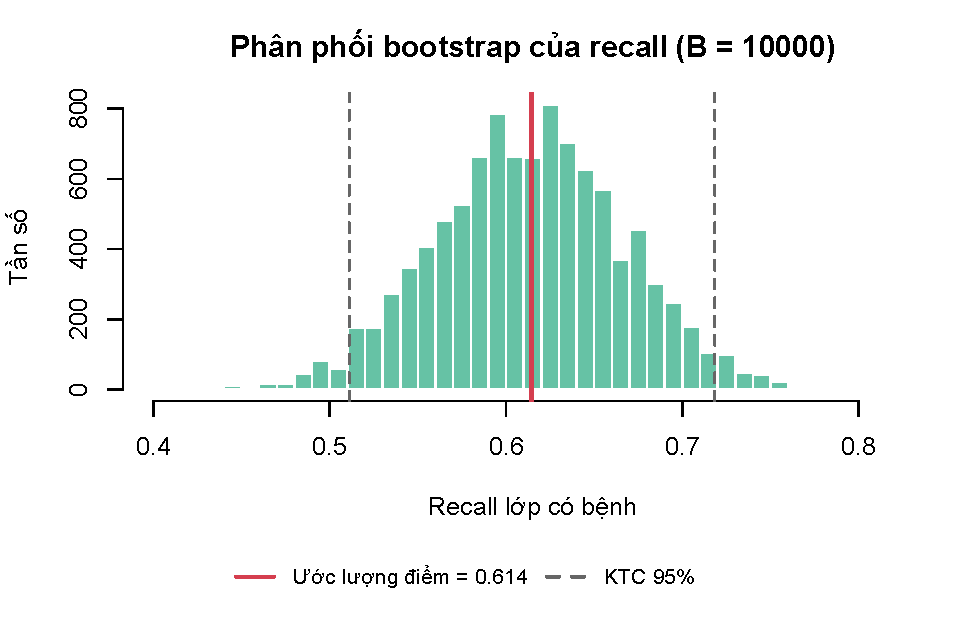
\includegraphics[width=\maxwidth]{figure/tl-boot-hist-1} 

}

\caption[Phân phối bootstrap của Recall lớp có bệnh với B = 10000]{Phân phối bootstrap của Recall lớp có bệnh với B = 10000}\label{fig:boot-hist}
\end{figure}

\end{knitrout}

Với ngưỡng mặc định $0{,}5$, recall lớp có bệnh là $0{,}614$ và khoảng tin
cậy 90\% là $[0{,}526;\ 0{,}700]$ --- bề rộng $0{,}174$, tức gần 17 điểm
phần trăm. Con số này đáng chú ý: nó có nghĩa là nếu chỉ báo cáo
``recall $= 0{,}61$'' thì ta đã che giấu một mức bất định rất lớn, hoàn
toàn do cỡ mẫu kiểm tra chỉ có 116 quan sát, trong đó 83 ca bệnh. Đây
chính là loại thông tin mà một con số điểm ước lượng đơn lẻ không bao giờ
truyền tải được. Hình~\ref{fig:boot-hist} cho thấy phân phối bootstrap
tương đối cân đối, biện minh cho việc dùng khoảng tin cậy phân vị đơn giản
thay vì BCa.

\section{Stratified K-fold Cross-Validation}

Phần trên đánh giá mô hình trên một lần chia 80/20 duy nhất. K-fold CV
luân phiên vai trò của cả 5 phần, nhờ đó mọi quan sát đều được dự đoán
đúng một lần bởi một mô hình chưa từng thấy nó.

Chọn $k = 5$ có lý do cụ thể: mỗi fold kiểm tra đúng 20\% dữ liệu, trùng
với tỉ lệ 80:20 ở phần trước, nên hai phần cùng đánh giá mô hình được huấn
luyện trên khoảng 466 mẫu và có thể so sánh trực tiếp với nhau.

\begin{knitrout}\scriptsize
\definecolor{shadecolor}{rgb}{0.969, 0.969, 0.969}\color{fgcolor}\begin{kframe}
\begin{alltt}
\hldef{K} \hlkwb{<-} \hlnum{5}
\hldef{folds} \hlkwb{<-} \hlkwd{stratified_folds}\hldef{(y_all,} \hlkwc{k} \hldef{= K,} \hlkwc{seed} \hldef{=} \hlnum{42}\hldef{)}

\hldef{cv_results} \hlkwb{<-} \hlkwd{data.frame}\hldef{()}
\hlkwa{for} \hldef{(i} \hlkwa{in} \hlkwd{seq_len}\hldef{(K)) \{}
  \hldef{te} \hlkwb{<-} \hlkwd{which}\hldef{(folds} \hlopt{==} \hldef{i)}
  \hldef{tr} \hlkwb{<-} \hlkwd{which}\hldef{(folds} \hlopt{!=} \hldef{i)}

  \hldef{fit_i} \hlkwb{<-} \hlkwd{fit_pipeline}\hldef{(X_all[tr, ,} \hlkwc{drop} \hldef{=} \hlnum{FALSE}\hldef{], y_all[tr],}
                        \hlkwc{lambda} \hldef{=} \hlnum{1}\hldef{,} \hlkwc{smote_k} \hldef{=} \hlnum{5}\hldef{)}
  \hldef{pred_i} \hlkwb{<-} \hlkwd{as.integer}\hldef{(}\hlkwd{pipeline_proba}\hldef{(fit_i,}
                                      \hldef{X_all[te, ,} \hlkwc{drop} \hldef{=} \hlnum{FALSE}\hldef{])} \hlopt{>=} \hlnum{0.5}\hldef{)}

  \hldef{m} \hlkwb{<-} \hlkwd{compute_metrics}\hldef{(y_all[te], pred_i)}
  \hldef{cv_results} \hlkwb{<-} \hlkwd{rbind}\hldef{(cv_results,} \hlkwd{data.frame}\hldef{(}
    \hlkwc{Fold} \hldef{= i,} \hlkwc{n_train} \hldef{=} \hlkwd{length}\hldef{(tr),} \hlkwc{n_test} \hldef{=} \hlkwd{length}\hldef{(te),}
    \hlkwc{Accuracy} \hldef{= m[}\hlsng{"accuracy"}\hldef{],} \hlkwc{Recall} \hldef{= m[}\hlsng{"recall1"}\hldef{],}
    \hlkwc{Macro_F1} \hldef{= m[}\hlsng{"macro_f1"}\hldef{]}
  \hldef{))}
\hldef{\}}
\hlkwd{rownames}\hldef{(cv_results)} \hlkwb{<-} \hlkwa{NULL}
\hlkwd{print}\hldef{(}\hlkwd{round}\hldef{(cv_results,} \hlnum{4}\hldef{),} \hlkwc{row.names} \hldef{=} \hlnum{FALSE}\hldef{)}
\end{alltt}
\begin{verbatim}
##  Fold n_train n_test Accuracy Recall Macro_F1
##     1     465    118   0.6186 0.5238   0.6124
##     2     466    117   0.6923 0.6386   0.6776
##     3     467    116   0.6466 0.6145   0.6263
##     4     467    116   0.6466 0.6265   0.6230
##     5     467    116   0.6897 0.6265   0.6758
\end{verbatim}
\begin{alltt}
\hlkwa{for} \hldef{(m} \hlkwa{in} \hlkwd{c}\hldef{(}\hlsng{"Accuracy"}\hldef{,} \hlsng{"Recall"}\hldef{,} \hlsng{"Macro_F1"}\hldef{)) \{}
  \hlkwd{cat}\hldef{(}\hlkwd{sprintf}\hldef{(}\hlsng{"  %-9s = %.3f +/- %.3f\textbackslash{}n"}\hldef{,}
              \hldef{m,} \hlkwd{mean}\hldef{(cv_results[[m]]),} \hlkwd{sd}\hldef{(cv_results[[m]])))}
\hldef{\}}
\end{alltt}
\begin{verbatim}
##   Accuracy  = 0.659 +/- 0.032
##   Recall    = 0.606 +/- 0.047
##   Macro_F1  = 0.643 +/- 0.031
\end{verbatim}
\end{kframe}
\end{knitrout}

Kết quả được báo cáo dạng \emph{trung bình $\pm$ độ lệch chuẩn giữa các
fold}, không phải một con số đơn lẻ. Độ lệch chuẩn ở đây có ý nghĩa riêng:
nó cho biết kết quả dao động bao nhiêu khi đổi sang một cách chia dữ liệu
khác. Recall dao động mạnh nhất ($0{,}606 \pm 0{,}047$, trải từ $0{,}524$
ở fold 1 tới $0{,}639$ ở fold 2), trong khi macro F1 ổn định hơn
($0{,}643 \pm 0{,}031$).

Điểm đáng chú ý là recall trung bình qua 5 fold ($0{,}606$) rất gần với
recall đo trên một lần chia 80/20 ở phần trước ($0{,}614$), và cả hai đều
nằm gọn trong khoảng tin cậy bootstrap $[0{,}526;\ 0{,}700]$. Hai phương
pháp resampling độc lập cho kết quả nhất quán --- một dấu hiệu tốt cho
thấy ước lượng không phải sản phẩm của một lần chia may mắn.

\section{Tinh chỉnh siêu tham số bằng grid search + K-fold}

Từ đây trở đi, quy trình tuân thủ nghiêm ngặt nguyên tắc phân vai:
\textbf{K-fold CV chạy trên tập huấn luyện để tinh chỉnh, tập kiểm tra bị
niêm phong} và chỉ được mở ở phần cuối cùng.

Hai siêu tham số được dò: cường độ điều chuẩn $\lambda$ của ridge và số
láng giềng $k$ mà SMOTE dùng để nội suy. Tiêu chí chấm điểm là macro F1
chứ \emph{không} phải recall thuần --- tối đa hoá recall lớp 1 có một
nghiệm tầm thường là dự đoán tất cả đều ``có bệnh'', cho recall bằng 1
nhưng hoàn toàn vô dụng.

\begin{knitrout}\scriptsize
\definecolor{shadecolor}{rgb}{0.969, 0.969, 0.969}\color{fgcolor}\begin{kframe}
\begin{alltt}
\hldef{param_grid} \hlkwb{<-} \hlkwd{expand.grid}\hldef{(}
  \hlkwc{lambda}  \hldef{=} \hlkwd{c}\hldef{(}\hlnum{0.01}\hldef{,} \hlnum{0.1}\hldef{,} \hlnum{1}\hldef{,} \hlnum{10}\hldef{,} \hlnum{100}\hldef{),}   \hlcom{# cường độ điều chuẩn ridge}
  \hlkwc{smote_k} \hldef{=} \hlkwd{c}\hldef{(}\hlnum{3}\hldef{,} \hlnum{5}\hldef{,} \hlnum{7}\hldef{)}                  \hlcom{# số láng giềng SMOTE}
\hldef{)}

\hldef{folds_inner} \hlkwb{<-} \hlkwd{stratified_folds}\hldef{(y_train,} \hlkwc{k} \hldef{=} \hlnum{5}\hldef{,} \hlkwc{seed} \hldef{=} \hlnum{42}\hldef{)}

\hldef{grid_mean} \hlkwb{<-} \hldef{grid_sd} \hlkwb{<-} \hlkwd{numeric}\hldef{(}\hlkwd{nrow}\hldef{(param_grid))}
\hlkwa{for} \hldef{(g} \hlkwa{in} \hlkwd{seq_len}\hldef{(}\hlkwd{nrow}\hldef{(param_grid))) \{}
  \hldef{scores} \hlkwb{<-} \hlkwd{numeric}\hldef{(}\hlnum{5}\hldef{)}
  \hlkwa{for} \hldef{(i} \hlkwa{in} \hlkwd{seq_len}\hldef{(}\hlnum{5}\hldef{)) \{}
    \hldef{te} \hlkwb{<-} \hlkwd{which}\hldef{(folds_inner} \hlopt{==} \hldef{i); tr} \hlkwb{<-} \hlkwd{which}\hldef{(folds_inner} \hlopt{!=} \hldef{i)}
    \hldef{fit_g} \hlkwb{<-} \hlkwd{fit_pipeline}\hldef{(X_train[tr, ,} \hlkwc{drop} \hldef{=} \hlnum{FALSE}\hldef{], y_train[tr],}
                          \hlkwc{lambda} \hldef{= param_grid}\hlopt{$}\hldef{lambda[g],}
                          \hlkwc{smote_k} \hldef{= param_grid}\hlopt{$}\hldef{smote_k[g])}
    \hldef{pred_g} \hlkwb{<-} \hlkwd{as.integer}\hldef{(}\hlkwd{pipeline_proba}\hldef{(}
      \hldef{fit_g, X_train[te, ,} \hlkwc{drop} \hldef{=} \hlnum{FALSE}\hldef{])} \hlopt{>=} \hlnum{0.5}\hldef{)}
    \hldef{scores[i]} \hlkwb{<-} \hlkwd{compute_metrics}\hldef{(y_train[te], pred_g)[}\hlsng{"macro_f1"}\hldef{]}
  \hldef{\}}
  \hldef{grid_mean[g]} \hlkwb{<-} \hlkwd{mean}\hldef{(scores)}
  \hldef{grid_sd[g]} \hlkwb{<-} \hlkwd{sd}\hldef{(scores)}     \hlcom{# dao động giữa 5 fold, dùng để đo mức nhiễu}
\hldef{\}}

\hldef{param_grid}\hlopt{$}\hldef{macro_f1} \hlkwb{<-} \hldef{grid_mean}
\hldef{param_grid}\hlopt{$}\hldef{sd_fold} \hlkwb{<-} \hldef{grid_sd}

\hlkwd{print}\hldef{(}\hlkwd{head}\hldef{(param_grid[}\hlkwd{order}\hldef{(}\hlopt{-}\hldef{param_grid}\hlopt{$}\hldef{macro_f1), ],} \hlnum{5}\hldef{),} \hlkwc{row.names} \hldef{=} \hlnum{FALSE}\hldef{)}
\end{alltt}
\begin{verbatim}
##  lambda smote_k  macro_f1    sd_fold
##     100       7 0.6440162 0.01687905
##     100       5 0.6408597 0.01098893
##     100       3 0.6407688 0.01654468
##       1       7 0.6406804 0.03143136
##      10       7 0.6398884 0.02943170
\end{verbatim}
\end{kframe}
\end{knitrout}

\subsection{Quy tắc phá thế hoà trong phạm vi một sai số chuẩn}

Lấy thẳng \texttt{which.max} là một sai lầm phổ biến khi các bộ tham số
cho điểm chênh nhau ít hơn chính sai số của phép đo. Ở đây bộ đứng đầu đạt
macro F1 $= 0{,}6440$ còn bộ thứ năm đạt $0{,}6399$ --- chênh lệch
$0{,}004$, trong khi sai số chuẩn của trung bình 5 fold là $0{,}0075$.
Trong tình huống đó, ``bộ thắng'' chỉ đơn giản là bộ gặp may với cách chia
fold cụ thể này; chọn nó không có cơ sở thống kê nào.

Cách xử lý: coi mọi bộ nằm trong phạm vi \emph{một sai số chuẩn} quanh
điểm cao nhất là ngang tài nhau, rồi phá hoà bằng một tiêu chí có lý do rõ
ràng.

\begin{knitrout}\scriptsize
\definecolor{shadecolor}{rgb}{0.969, 0.969, 0.969}\color{fgcolor}\begin{kframe}
\begin{alltt}
\hldef{i_top} \hlkwb{<-} \hlkwd{which.max}\hldef{(param_grid}\hlopt{$}\hldef{macro_f1)}
\hldef{se_top} \hlkwb{<-} \hldef{param_grid}\hlopt{$}\hldef{sd_fold[i_top]} \hlopt{/} \hlkwd{sqrt}\hldef{(}\hlnum{5}\hldef{)}   \hlcom{# sai số chuẩn của trung bình}
\hldef{tied} \hlkwb{<-} \hlkwd{which}\hldef{(param_grid}\hlopt{$}\hldef{macro_f1} \hlopt{>=} \hldef{param_grid}\hlopt{$}\hldef{macro_f1[i_top]} \hlopt{-} \hldef{se_top)}

\hldef{cand} \hlkwb{<-} \hldef{tied[param_grid}\hlopt{$}\hldef{lambda[tied]} \hlopt{==} \hlkwd{min}\hldef{(param_grid}\hlopt{$}\hldef{lambda[tied])]}
\hldef{best_idx} \hlkwb{<-} \hldef{cand[}\hlkwd{which.max}\hldef{(param_grid}\hlopt{$}\hldef{macro_f1[cand])]}
\hldef{best} \hlkwb{<-} \hldef{param_grid[best_idx, ]}

\hlkwd{cat}\hldef{(}\hlkwd{sprintf}\hldef{(}\hlsng{"Điểm cao nhất: %.4f (lambda = %g), sai số chuẩn = %.4f\textbackslash{}n"}\hldef{,}
            \hldef{param_grid}\hlopt{$}\hldef{macro_f1[i_top], param_grid}\hlopt{$}\hldef{lambda[i_top], se_top))}
\end{alltt}
\begin{verbatim}
## Điểm cao nhất: 0.6440 (lambda = 100), sai số chuẩn = 0.0075
\end{verbatim}
\begin{alltt}
\hlkwd{cat}\hldef{(}\hlkwd{sprintf}\hldef{(}\hlsng{"Có %d/%d bộ nằm trong phạm vi một sai số chuẩn\textbackslash{}n"}\hldef{,}
            \hlkwd{length}\hldef{(tied),} \hlkwd{nrow}\hldef{(param_grid)))}
\end{alltt}
\begin{verbatim}
## Có 14/15 bộ nằm trong phạm vi một sai số chuẩn
\end{verbatim}
\begin{alltt}
\hlkwd{cat}\hldef{(}\hlkwd{sprintf}\hldef{(}\hlsng{"Phá hoà bằng lambda nhỏ nhất -> lambda = %g, smote_k = %g\textbackslash{}n"}\hldef{,}
            \hldef{best}\hlopt{$}\hldef{lambda, best}\hlopt{$}\hldef{smote_k))}
\end{alltt}
\begin{verbatim}
## Phá hoà bằng lambda nhỏ nhất -> lambda = 0.01, smote_k = 3
\end{verbatim}
\begin{alltt}
\hlkwd{cat}\hldef{(}\hlkwd{sprintf}\hldef{(}\hlsng{"Đã thử %d bộ x 5 fold = %d lần khớp mô hình\textbackslash{}n"}\hldef{,}
            \hlkwd{nrow}\hldef{(param_grid),} \hlkwd{nrow}\hldef{(param_grid)} \hlopt{*} \hlnum{5}\hldef{))}
\end{alltt}
\begin{verbatim}
## Đã thử 15 bộ x 5 fold = 75 lần khớp mô hình
\end{verbatim}
\end{kframe}
\end{knitrout}

Kết quả cho thấy 14 trên 15 bộ tham số nằm trong phạm vi một sai số chuẩn
--- nói cách khác, lưới tham số này gần như không phân biệt được các cấu
hình với nhau, và bất kỳ lựa chọn nào dựa trên chênh lệch điểm số đều là
lựa chọn dựa trên nhiễu.

Tiêu chí phá hoà được dùng là \textbf{chọn $\lambda$ nhỏ nhất}. Cần nhấn
mạnh rằng điều này \emph{ngược} với quy tắc 1-SE quen thuộc trong tài
liệu, vốn ưu tiên mô hình điều chuẩn mạnh hơn cho gọn. Lý do đảo chiều nằm
ở bước tiếp theo của quy trình: ta sẽ chỉnh ngưỡng phân loại, mà việc đó
cần xác suất dự đoán trải rộng. $\lambda$ lớn nén các hệ số lại, kéo xác
suất co về quanh $0{,}5$, khiến ngưỡng trở nên cực kỳ nhạy --- dịch một
chút là recall của hai lớp đảo lộn. Khi các bộ đã ngang điểm nhau trong
phạm vi nhiễu, chọn bộ cho xác suất trải rộng hơn là lựa chọn có căn cứ.

\section{Chọn ngưỡng phân loại}

Ngưỡng mặc định $0{,}5$ tối ưu cho độ chính xác tổng thể và không ưu tiên
lớp nào. Bài toán y tế thì khác: bỏ sót một ca bệnh (FN) tốn kém hơn nhiều
so với báo động nhầm một người khoẻ (FP), vì FP chỉ dẫn tới một xét nghiệm
bổ sung còn FN có thể khiến bệnh tiến triển không được phát hiện. Vì vậy
ta hạ ngưỡng xuống để đẩy recall lớp có bệnh lên.

Ngưỡng \emph{phải} được dò trên tập huấn luyện. Dò trên tập kiểm tra thì
tập kiểm tra đã tham gia vào một quyết định, và con số báo cáo cuối cùng
sẽ lạc quan giả tạo. Ta dùng dự đoán \emph{out-of-fold}: mỗi mẫu huấn
luyện được chấm điểm bởi mô hình chưa từng nhìn thấy nó.

\begin{knitrout}\scriptsize
\definecolor{shadecolor}{rgb}{0.969, 0.969, 0.969}\color{fgcolor}\begin{kframe}
\begin{alltt}
\hldef{oof_proba} \hlkwb{<-} \hlkwd{numeric}\hldef{(}\hlkwd{length}\hldef{(y_train))}
\hlkwa{for} \hldef{(i} \hlkwa{in} \hlkwd{seq_len}\hldef{(}\hlnum{5}\hldef{)) \{}
  \hldef{te} \hlkwb{<-} \hlkwd{which}\hldef{(folds_inner} \hlopt{==} \hldef{i); tr} \hlkwb{<-} \hlkwd{which}\hldef{(folds_inner} \hlopt{!=} \hldef{i)}
  \hldef{fit_o} \hlkwb{<-} \hlkwd{fit_pipeline}\hldef{(X_train[tr, ,} \hlkwc{drop} \hldef{=} \hlnum{FALSE}\hldef{], y_train[tr],}
                        \hlkwc{lambda} \hldef{= best}\hlopt{$}\hldef{lambda,} \hlkwc{smote_k} \hldef{= best}\hlopt{$}\hldef{smote_k)}
  \hldef{oof_proba[te]} \hlkwb{<-} \hlkwd{pipeline_proba}\hldef{(fit_o, X_train[te, ,} \hlkwc{drop} \hldef{=} \hlnum{FALSE}\hldef{])}
\hldef{\}}

\hldef{grid_thr} \hlkwb{<-} \hlkwd{seq}\hldef{(}\hlnum{0.05}\hldef{,} \hlnum{0.95}\hldef{,} \hlkwc{by} \hldef{=} \hlnum{0.005}\hldef{)}
\hldef{rec1} \hlkwb{<-} \hldef{rec0} \hlkwb{<-} \hlkwd{numeric}\hldef{(}\hlkwd{length}\hldef{(grid_thr))}
\hlkwa{for} \hldef{(i} \hlkwa{in} \hlkwd{seq_along}\hldef{(grid_thr)) \{}
  \hldef{m} \hlkwb{<-} \hlkwd{compute_metrics}\hldef{(y_train,} \hlkwd{as.integer}\hldef{(oof_proba} \hlopt{>=} \hldef{grid_thr[i]))}
  \hldef{rec1[i]} \hlkwb{<-} \hldef{m[}\hlsng{"recall1"}\hldef{]; rec0[i]} \hlkwb{<-} \hldef{m[}\hlsng{"recall0"}\hldef{]}
\hldef{\}}
\end{alltt}
\end{kframe}
\end{knitrout}

\begin{knitrout}\scriptsize
\definecolor{shadecolor}{rgb}{0.969, 0.969, 0.969}\color{fgcolor}\begin{kframe}
\begin{alltt}
\hlkwd{plot}\hldef{(grid_thr, rec1,} \hlkwc{type} \hldef{=} \hlsng{"l"}\hldef{,} \hlkwc{col} \hldef{=} \hlsng{"#d53e4f"}\hldef{,} \hlkwc{lwd} \hldef{=} \hlnum{2}\hldef{,} \hlkwc{ylim} \hldef{=} \hlkwd{c}\hldef{(}\hlnum{0}\hldef{,} \hlnum{1}\hldef{),}
     \hlkwc{xlab} \hldef{=} \hlsng{"Ngưỡng phân loại"}\hldef{,} \hlkwc{ylab} \hldef{=} \hlsng{"Recall"}\hldef{,}
     \hlkwc{main} \hldef{=} \hlsng{"Recall hai lớp theo ngưỡng (out-of-fold trên tập train)"}\hldef{)}
\hlkwd{lines}\hldef{(grid_thr, rec0,} \hlkwc{col} \hldef{=} \hlsng{"#3288bd"}\hldef{,} \hlkwc{lwd} \hldef{=} \hlnum{2}\hldef{)}
\hlkwd{abline}\hldef{(}\hlkwc{v} \hldef{=} \hlnum{0.5}\hldef{,} \hlkwc{col} \hldef{=} \hlsng{"gray50"}\hldef{,} \hlkwc{lty} \hldef{=} \hlnum{3}\hldef{)}
\hlkwd{grid}\hldef{(}\hlkwc{col} \hldef{=} \hlsng{"gray90"}\hldef{)}
\hlkwd{legend}\hldef{(}\hlsng{"right"}\hldef{,} \hlkwc{bty} \hldef{=} \hlsng{"n"}\hldef{,} \hlkwc{cex} \hldef{=} \hlnum{0.85}\hldef{,} \hlkwc{lwd} \hldef{=} \hlnum{2}\hldef{,}
       \hlkwc{legend} \hldef{=} \hlkwd{c}\hldef{(}\hlsng{"Recall lớp 1 - có bệnh (độ nhạy)"}\hldef{,}
                  \hlsng{"Recall lớp 0 - không bệnh (độ đặc hiệu)"}\hldef{,}
                  \hlsng{"Ngưỡng mặc định 0.5"}\hldef{),}
       \hlkwc{col} \hldef{=} \hlkwd{c}\hldef{(}\hlsng{"#d53e4f"}\hldef{,} \hlsng{"#3288bd"}\hldef{,} \hlsng{"gray50"}\hldef{),} \hlkwc{lty} \hldef{=} \hlkwd{c}\hldef{(}\hlnum{1}\hldef{,} \hlnum{1}\hldef{,} \hlnum{3}\hldef{))}
\end{alltt}
\end{kframe}\begin{figure}

{\centering 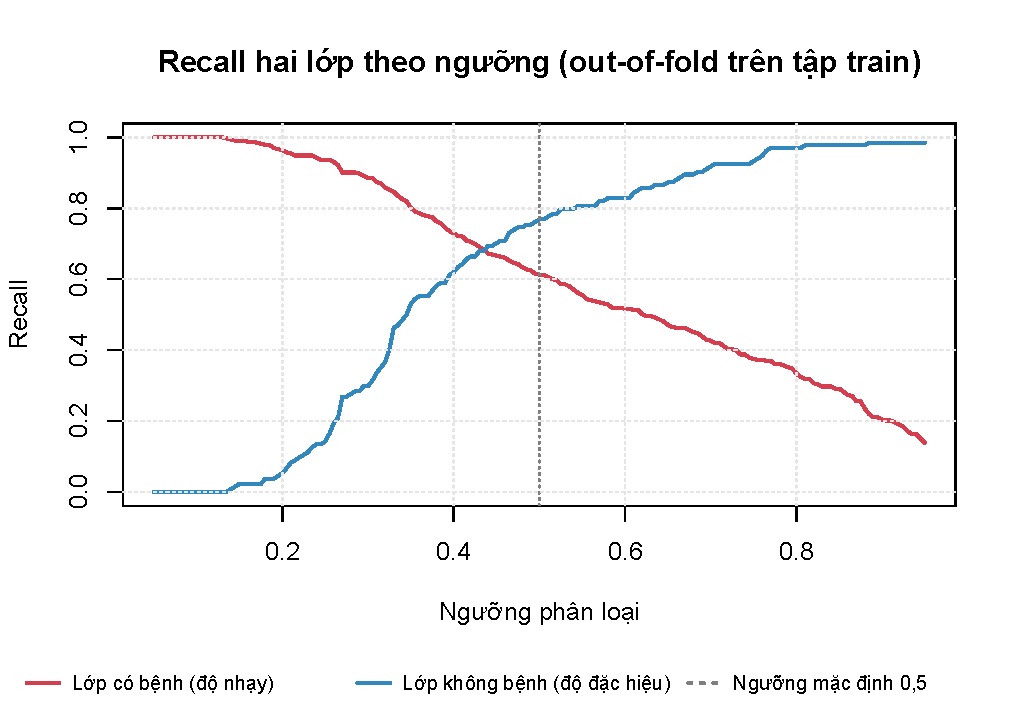
\includegraphics[width=\maxwidth]{figure/tl-threshold-plot-1} 

}

\caption[Đánh đổi giữa độ nhạy và độ đặc hiệu khi thay đổi ngưỡng phân loại]{Đánh đổi giữa độ nhạy và độ đặc hiệu khi thay đổi ngưỡng phân loại}\label{fig:threshold-plot}
\end{figure}

\end{knitrout}

Hình~\ref{fig:threshold-plot} thể hiện đúng bản chất đánh đổi: hai đường
đi ngược chiều nhau, mọi điểm recall lớp 1 tăng thêm đều phải trả bằng
recall lớp 0 giảm đi. Bảng tra dưới đây lượng hoá cái giá đó.

\begin{knitrout}\scriptsize
\definecolor{shadecolor}{rgb}{0.969, 0.969, 0.969}\color{fgcolor}\begin{kframe}
\begin{alltt}
\hldef{lookup} \hlkwb{<-} \hlkwd{data.frame}\hldef{()}
\hlkwa{for} \hldef{(target} \hlkwa{in} \hlkwd{c}\hldef{(}\hlnum{0.70}\hldef{,} \hlnum{0.75}\hldef{,} \hlnum{0.80}\hldef{,} \hlnum{0.85}\hldef{,} \hlnum{0.90}\hldef{,} \hlnum{0.95}\hldef{)) \{}
  \hldef{ok} \hlkwb{<-} \hlkwd{which}\hldef{(rec1} \hlopt{>=} \hldef{target)}
  \hlkwa{if} \hldef{(}\hlkwd{length}\hldef{(ok)} \hlopt{==} \hlnum{0}\hldef{)} \hlkwa{next}
  \hldef{i} \hlkwb{<-} \hldef{ok[}\hlkwd{which.max}\hldef{(grid_thr[ok])]}     \hlcom{# ngưỡng CAO NHẤT vẫn đạt mục tiêu}
  \hldef{lookup} \hlkwb{<-} \hlkwd{rbind}\hldef{(lookup,} \hlkwd{data.frame}\hldef{(}
    \hlkwc{recall_muc_tieu} \hldef{= target,} \hlkwc{nguong} \hldef{= grid_thr[i],}
    \hlkwc{recall_lop1} \hldef{= rec1[i],} \hlkwc{recall_lop0} \hldef{= rec0[i]}
  \hldef{))}
\hldef{\}}
\hlkwd{print}\hldef{(}\hlkwd{round}\hldef{(lookup,} \hlnum{3}\hldef{),} \hlkwc{row.names} \hldef{=} \hlnum{FALSE}\hldef{)}
\end{alltt}
\begin{verbatim}
##  recall_muc_tieu nguong recall_lop1 recall_lop0
##             0.70  0.420       0.706       0.664
##             0.75  0.385       0.757       0.590
##             0.80  0.350       0.802       0.530
##             0.85  0.325       0.853       0.403
##             0.90  0.285       0.901       0.284
##             0.95  0.210       0.955       0.082
\end{verbatim}
\begin{alltt}
\hldef{TARGET_RECALL} \hlkwb{<-} \hlnum{0.70}
\hldef{ok} \hlkwb{<-} \hlkwd{which}\hldef{(rec1} \hlopt{>=} \hldef{TARGET_RECALL)}
\hldef{threshold} \hlkwb{<-} \hldef{grid_thr[ok[}\hlkwd{which.max}\hldef{(grid_thr[ok])]]}

\hlkwd{cat}\hldef{(}\hlkwd{sprintf}\hldef{(}\hlsng{"\textbackslash{}nNgưỡng mặc định : 0.500\textbackslash{}n"}\hldef{))}
\end{alltt}
\begin{verbatim}
## 
## Ngưỡng mặc định : 0.500
\end{verbatim}
\begin{alltt}
\hlkwd{cat}\hldef{(}\hlkwd{sprintf}\hldef{(}\hlsng{"Ngưỡng đã chọn  : %.3f  (mục tiêu recall >= %.2f)\textbackslash{}n"}\hldef{,}
            \hldef{threshold, TARGET_RECALL))}
\end{alltt}
\begin{verbatim}
## Ngưỡng đã chọn  : 0.420  (mục tiêu recall >= 0.70)
\end{verbatim}
\end{kframe}
\end{knitrout}

Bảng tra cho thấy cái giá tăng rất nhanh. Để đạt recall $0{,}70$ ta chỉ
mất một ít độ đặc hiệu (còn $0{,}664$); nhưng để đạt $0{,}90$ thì độ đặc
hiệu tụt xuống $0{,}284$, và ở mức $0{,}95$ chỉ còn $0{,}082$ --- lúc đó
mô hình gần như báo ``có bệnh'' cho tất cả mọi người và mất hết giá trị
sàng lọc. Mức $0{,}70$ được chọn vì nó nằm ở đoạn đánh đổi còn cân bằng,
tương ứng ngưỡng $0{,}420$.

\section{Đánh giá cuối cùng trên tập kiểm tra}

Đây là lần \textbf{đầu tiên} tập kiểm tra được đụng tới kể từ khi niêm
phong. Mô hình được khớp lại trên toàn bộ tập huấn luyện với siêu tham số
đã chọn, rồi áp ngưỡng $0{,}420$.

\begin{knitrout}\scriptsize
\definecolor{shadecolor}{rgb}{0.969, 0.969, 0.969}\color{fgcolor}\begin{kframe}
\begin{alltt}
\hldef{fit_best} \hlkwb{<-} \hlkwd{fit_pipeline}\hldef{(X_train, y_train,}
                         \hlkwc{lambda} \hldef{= best}\hlopt{$}\hldef{lambda,} \hlkwc{smote_k} \hldef{= best}\hlopt{$}\hldef{smote_k)}
\hldef{proba_final} \hlkwb{<-} \hlkwd{pipeline_proba}\hldef{(fit_best, X_test)}
\hldef{pred_final} \hlkwb{<-} \hlkwd{as.integer}\hldef{(proba_final} \hlopt{>=} \hldef{threshold)}
\hldef{pred_05} \hlkwb{<-} \hlkwd{as.integer}\hldef{(proba_final} \hlopt{>=} \hlnum{0.5}\hldef{)}

\hldef{m_final} \hlkwb{<-} \hlkwd{print_confusion}\hldef{(y_test, pred_final,}
                           \hlkwd{sprintf}\hldef{(}\hlsng{"CONFUSION MATRIX (ngưỡng %.3f)"}\hldef{,}
                                   \hldef{threshold))}
\end{alltt}
\begin{verbatim}
## 
## CONFUSION MATRIX (ngưỡng 0.420)
##             Dự đoán
## Thực tế  Không bệnh Có bệnh
##   Không bệnh         27       6
##   Có bệnh            25      58
##   TN =  27   không bệnh, đoán đúng
##   FP =   6   không bệnh nhưng báo có bệnh
##   FN =  25   CÓ BỆNH nhưng bỏ sót
##   TP =  58   có bệnh, bắt được
\end{verbatim}
\begin{alltt}
\hlkwd{cat}\hldef{(}\hlsng{"\textbackslash{}nCác chỉ số trên tập test:\textbackslash{}n"}\hldef{)}
\end{alltt}
\begin{verbatim}
## 
## Các chỉ số trên tập test:
\end{verbatim}
\begin{alltt}
\hlkwd{print}\hldef{(}\hlkwd{round}\hldef{(m_final,} \hlnum{3}\hldef{))}
\end{alltt}
\begin{verbatim}
##   accuracy    recall1 precision1    recall0 precision0   macro_f1 
##      0.733      0.699      0.906      0.818      0.519      0.712
\end{verbatim}
\end{kframe}
\end{knitrout}

\begin{knitrout}\scriptsize
\definecolor{shadecolor}{rgb}{0.969, 0.969, 0.969}\color{fgcolor}\begin{kframe}
\begin{alltt}
\hldef{cmp} \hlkwb{<-} \hlkwd{rbind}\hldef{(}
  \hlkwc{`0.500 (mặc định)`} \hldef{=} \hlkwd{compute_metrics}\hldef{(y_test, pred_05),}
  \hlkwc{`đã chỉnh`}         \hldef{=} \hlkwd{compute_metrics}\hldef{(y_test, pred_final)}
\hldef{)}
\hlkwd{print}\hldef{(}\hlkwd{round}\hldef{(cmp,} \hlnum{3}\hldef{))}
\end{alltt}
\begin{verbatim}
##                  accuracy recall1 precision1 recall0 precision0
## 0.500 (mặc định)    0.681   0.614      0.911   0.848      0.467
## đã chỉnh            0.733   0.699      0.906   0.818      0.519
##                  macro_f1
## 0.500 (mặc định)    0.668
## đã chỉnh            0.712
\end{verbatim}
\end{kframe}
\end{knitrout}

Việc hạ ngưỡng từ $0{,}500$ xuống $0{,}420$ đẩy recall lớp có bệnh từ
$0{,}614$ lên $0{,}699$ --- bắt thêm được 7 ca bệnh --- với cái giá là độ
đặc hiệu giảm nhẹ từ $0{,}848$ xuống $0{,}818$ (thêm 1 báo động nhầm).
Điều đáng chú ý là accuracy và macro F1 \emph{cũng} tăng, chứ không giảm
như thường thấy khi ưu tiên một lớp. Nguyên nhân là ngưỡng $0{,}5$ vốn
không tối ưu trên dữ liệu mất cân bằng này ngay cả theo tiêu chí tổng hợp;
mức $0{,}420$ tình cờ tốt hơn ở cả hai phương diện.

\subsection{Khoảng tin cậy bootstrap cho toàn bộ chỉ số}

\begin{knitrout}\scriptsize
\definecolor{shadecolor}{rgb}{0.969, 0.969, 0.969}\color{fgcolor}\begin{kframe}
\begin{alltt}
\hldef{CONF2} \hlkwb{<-} \hlnum{0.95}
\hldef{B2} \hlkwb{<-} \hlnum{2000}
\hldef{boot_mat} \hlkwb{<-} \hlkwd{matrix}\hldef{(}\hlnum{NA}\hldef{,} \hlkwc{nrow} \hldef{= B2,} \hlkwc{ncol} \hldef{=} \hlkwd{length}\hldef{(m_final),}
                   \hlkwc{dimnames} \hldef{=} \hlkwd{list}\hldef{(}\hlkwa{NULL}\hldef{,} \hlkwd{names}\hldef{(m_final)))}

\hlkwa{for} \hldef{(b} \hlkwa{in} \hlkwd{seq_len}\hldef{(B2)) \{}
  \hldef{idx} \hlkwb{<-} \hlkwd{sample.int}\hldef{(n_test, n_test,} \hlkwc{replace} \hldef{=} \hlnum{TRUE}\hldef{)}
  \hlkwa{if} \hldef{(}\hlkwd{length}\hldef{(}\hlkwd{unique}\hldef{(y_test[idx]))} \hlopt{<} \hlnum{2}\hldef{)} \hlkwa{next}     \hlcom{# mẫu suy biến, bỏ qua}
  \hldef{boot_mat[b, ]} \hlkwb{<-} \hlkwd{compute_metrics}\hldef{(y_test[idx], pred_final[idx])}
\hldef{\}}
\hldef{boot_mat} \hlkwb{<-} \hldef{boot_mat[}\hlkwd{complete.cases}\hldef{(boot_mat), ,} \hlkwc{drop} \hldef{=} \hlnum{FALSE}\hldef{]}

\hldef{tail2} \hlkwb{<-} \hldef{(}\hlnum{1} \hlopt{-} \hldef{CONF2)} \hlopt{/} \hlnum{2}
\hldef{ci_tbl} \hlkwb{<-} \hlkwd{data.frame}\hldef{(}
  \hlkwc{diem_uoc_luong} \hldef{= m_final,}
  \hlkwc{ci_duoi} \hldef{=} \hlkwd{apply}\hldef{(boot_mat,} \hlnum{2}\hldef{, quantile,} \hlkwc{probs} \hldef{= tail2),}
  \hlkwc{ci_tren} \hldef{=} \hlkwd{apply}\hldef{(boot_mat,} \hlnum{2}\hldef{, quantile,} \hlkwc{probs} \hldef{=} \hlnum{1} \hlopt{-} \hldef{tail2),}
  \hlkwc{sai_so_chuan} \hldef{=} \hlkwd{apply}\hldef{(boot_mat,} \hlnum{2}\hldef{, sd)}
\hldef{)}
\hlkwd{print}\hldef{(}\hlkwd{round}\hldef{(ci_tbl,} \hlnum{4}\hldef{))}
\end{alltt}
\begin{verbatim}
##            diem_uoc_luong ci_duoi ci_tren sai_so_chuan
## accuracy           0.7328  0.6552  0.8103       0.0413
## recall1            0.6988  0.5977  0.8000       0.0512
## precision1         0.9062  0.8305  0.9701       0.0368
## recall0            0.8182  0.6774  0.9412       0.0676
## precision0         0.5192  0.3859  0.6586       0.0693
## macro_f1           0.7122  0.6230  0.7947       0.0437
\end{verbatim}
\end{kframe}
\end{knitrout}

\begin{knitrout}\scriptsize
\definecolor{shadecolor}{rgb}{0.969, 0.969, 0.969}\color{fgcolor}\begin{kframe}
\begin{alltt}
\hlkwd{par}\hldef{(}\hlkwc{mar} \hldef{=} \hlkwd{c}\hldef{(}\hlnum{5}\hldef{,} \hlnum{9}\hldef{,} \hlnum{4}\hldef{,} \hlnum{2}\hldef{))}
\hldef{n_m} \hlkwb{<-} \hlkwd{nrow}\hldef{(ci_tbl)}
\hlkwd{plot}\hldef{(ci_tbl}\hlopt{$}\hldef{diem_uoc_luong,} \hlkwd{seq_len}\hldef{(n_m),} \hlkwc{pch} \hldef{=} \hlnum{19}\hldef{,} \hlkwc{col} \hldef{=} \hlsng{"#3288bd"}\hldef{,}
     \hlkwc{cex} \hldef{=} \hlnum{1.3}\hldef{,} \hlkwc{xlim} \hldef{=} \hlkwd{c}\hldef{(}\hlnum{0}\hldef{,} \hlnum{1}\hldef{),} \hlkwc{yaxt} \hldef{=} \hlsng{"n"}\hldef{,} \hlkwc{ylab} \hldef{=} \hlsng{""}\hldef{,} \hlkwc{xlab} \hldef{=} \hlsng{"Giá trị"}\hldef{,}
     \hlkwc{main} \hldef{=} \hlkwd{sprintf}\hldef{(}\hlsng{"Khoảng tin cậy bootstrap %.0f%%"}\hldef{, CONF2} \hlopt{*} \hlnum{100}\hldef{))}
\hlkwd{arrows}\hldef{(ci_tbl}\hlopt{$}\hldef{ci_duoi,} \hlkwd{seq_len}\hldef{(n_m), ci_tbl}\hlopt{$}\hldef{ci_tren,} \hlkwd{seq_len}\hldef{(n_m),}
       \hlkwc{length} \hldef{=} \hlnum{0.05}\hldef{,} \hlkwc{angle} \hldef{=} \hlnum{90}\hldef{,} \hlkwc{code} \hldef{=} \hlnum{3}\hldef{,} \hlkwc{col} \hldef{=} \hlsng{"gray40"}\hldef{)}
\hlkwd{axis}\hldef{(}\hlnum{2}\hldef{,} \hlkwd{seq_len}\hldef{(n_m),} \hlkwd{rownames}\hldef{(ci_tbl),} \hlkwc{las} \hldef{=} \hlnum{2}\hldef{,} \hlkwc{cex.axis} \hldef{=} \hlnum{0.85}\hldef{)}
\hlkwd{abline}\hldef{(}\hlkwc{v} \hldef{=} \hlnum{0.5}\hldef{,} \hlkwc{col} \hldef{=} \hlsng{"#d53e4f"}\hldef{,} \hlkwc{lty} \hldef{=} \hlnum{3}\hldef{)}
\end{alltt}
\end{kframe}\begin{figure}

{\centering 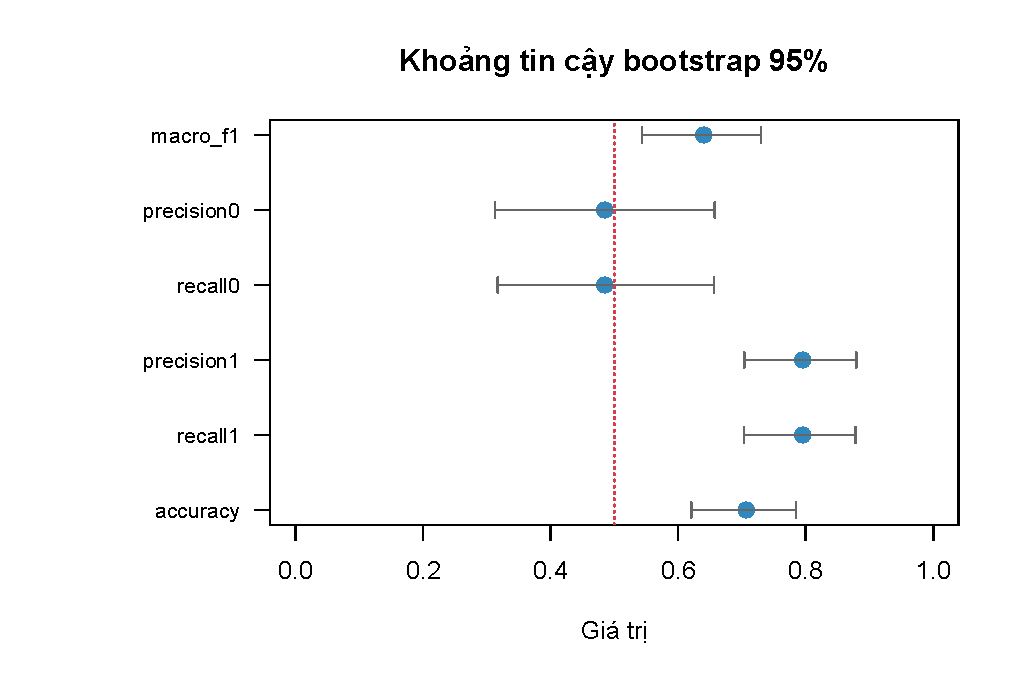
\includegraphics[width=\maxwidth]{figure/tl-forest-plot-1} 

}

\caption[Khoảng tin cậy bootstrap 95\% cho sáu chỉ số trên tập kiểm tra]{Khoảng tin cậy bootstrap 95\% cho sáu chỉ số trên tập kiểm tra}\label{fig:forest-plot}
\end{figure}

\begin{kframe}\begin{alltt}
\hlkwd{par}\hldef{(}\hlkwc{mar} \hldef{=} \hlkwd{c}\hldef{(}\hlnum{5}\hldef{,} \hlnum{4}\hldef{,} \hlnum{4}\hldef{,} \hlnum{2}\hldef{)} \hlopt{+} \hlnum{0.1}\hldef{)}
\end{alltt}
\end{kframe}
\end{knitrout}

Kết quả chính: \textbf{recall lớp có bệnh $= 0{,}699$, khoảng tin cậy 95\%
là $[0{,}598;\ 0{,}800]$}. Hình~\ref{fig:forest-plot} cho thấy độ rộng
khoảng tin cậy khác nhau đáng kể giữa các chỉ số, và sự khác biệt đó phản
ánh trực tiếp cỡ mẫu dùng để tính từng chỉ số. \texttt{precision1} có
khoảng hẹp nhất ($\pm 0{,}07$) vì mẫu số của nó gồm 64 dự đoán dương tính;
ngược lại \texttt{precision0} có khoảng rộng nhất ($[0{,}386;\ 0{,}659]$,
sai số chuẩn $0{,}069$) vì chỉ tính trên 52 dự đoán âm tính. Nói cách
khác, ước lượng $0{,}519$ cho \texttt{precision0} gần như không cho biết
điều gì chắc chắn --- một cảnh báo mà điểm ước lượng đơn lẻ hoàn toàn giấu
đi.

\section{Kết luận}

Tiểu luận đã xây dựng một quy trình phân loại hoàn chỉnh trên dữ liệu ILPD
và, quan trọng hơn, minh hoạ vai trò phân công rõ ràng giữa hai kỹ thuật
resampling.

\textbf{K-fold Cross-Validation trong vai trò chọn mô hình.} Kiểm định
chéo phân tầng 5 phần được dùng ở ba chỗ khác nhau: đánh giá tổng quát mô
hình cơ sở ($0{,}643 \pm 0{,}031$ macro F1), dò 15 bộ siêu tham số qua 75
lần khớp mô hình, và sinh dự đoán out-of-fold để chọn ngưỡng phân loại.
Điểm rút ra đáng giá nhất không phải bộ tham số thắng cuộc mà là phát hiện
rằng 14 trên 15 bộ nằm trong phạm vi một sai số chuẩn của nhau --- tức là
lưới tham số này về cơ bản không phân biệt được các cấu hình, và việc chọn
bộ có điểm cao nhất sẽ là chọn theo nhiễu. Chính độ lệch chuẩn giữa các
fold, thứ mà một lần chia train/test đơn lẻ không thể cung cấp, đã cho
phép nhận ra điều đó.

\textbf{Bootstrap trong vai trò định lượng độ tin cậy.} Mô hình cuối đạt
recall $0{,}699$ trên tập kiểm tra, nhưng khoảng tin cậy 95\% trải từ
$0{,}598$ tới $0{,}800$. Bề rộng hơn 20 điểm phần trăm này là thông tin
thiết yếu: nó nói rằng với cỡ mẫu hiện có, ta không thể phân biệt được mô
hình này với một mô hình có recall thật sự là $0{,}62$ hay $0{,}78$. Mọi
so sánh với các nghiên cứu khác trên cùng bộ dữ liệu đều phải đọc qua lăng
kính đó.

\textbf{Về mô hình.} Cấu hình cuối là hồi quy logistic ridge với
$\lambda = 0{,}01$, SMOTE với $k = 3$ láng giềng, ngưỡng phân loại
$0{,}420$, trên 7 biến còn lại sau khi loại \texttt{Direct\_Bilirubin}
(đa cộng tuyến), \texttt{Gender} và \texttt{Total\_Protiens} (không đạt
FDR). Nhóm biến quan trọng nhất là các men gan và bilirubin, với kích
thước ảnh hưởng rank-biserial khoảng $0{,}35$--$0{,}39$.

\subsection{Hạn chế}

\begin{enumerate}
  \item \textbf{Hiệu năng tuyệt đối còn thấp.} Recall $0{,}699$ nghĩa là
        vẫn bỏ sót khoảng 30\% ca bệnh (25 trên 83 bệnh nhân trong tập
        kiểm tra). Đặc biệt \texttt{precision0} chỉ đạt $0{,}519$: trong
        số những người mô hình kết luận là khoẻ mạnh, gần một nửa thực ra
        có bệnh. Đây chưa phải mức chấp nhận được cho một công cụ sàng lọc
        dùng trong thực tế.
  \item \textbf{Khoảng tin cậy bootstrap chỉ tính một nguồn bất định.} Vì
        mô hình được cố định trong suốt vòng lặp và chỉ tập kiểm tra được
        rút lại, khoảng thu được phản ánh biến thiên do lấy mẫu bệnh nhân
        kiểm tra, chứ không tính tới biến thiên do thay đổi tập huấn
        luyện. Độ bất định thật sự do đó \emph{rộng hơn} con số báo cáo.
        Khắc phục đúng cách là dùng bootstrap lồng --- huấn luyện lại mô
        hình trong mỗi lần lặp --- với chi phí tính toán cao hơn nhiều.
  \item \textbf{Cỡ mẫu nhỏ.} 583 quan sát, trong đó tập kiểm tra chỉ 116,
        là nguyên nhân trực tiếp của các khoảng tin cậy rộng.
  \item \textbf{Tính đại diện.} Dữ liệu thu thập ở một vùng địa lý duy
        nhất (đông bắc Andhra Pradesh, Ấn Độ) nên kết quả chưa chắc tổng
        quát hoá được sang quần thể khác.
  \item \textbf{Đa cộng tuyến còn sót.} \texttt{Albumin} và
        \texttt{Albumin\_and\_Globulin\_Ratio} vẫn liên quan chặt về định
        nghĩa; điều chuẩn ridge làm dịu vấn đề này nhưng không loại bỏ
        được nó, và hệ quả là các hệ số riêng lẻ của mô hình không nên
        được diễn giải như mức độ quan trọng của từng biến.
\end{enumerate}

\subsection{Hướng mở rộng}

Ba hướng có triển vọng nhất, xếp theo mức độ ưu tiên. Thứ nhất,
\emph{bootstrap lồng} để khoảng tin cậy bao gồm cả biến thiên do huấn
luyện. Thứ hai, \emph{repeated stratified k-fold} --- lặp toàn bộ quy
trình CV với nhiều seed khác nhau --- để giảm phương sai của ước lượng và
kiểm tra xem kết luận ``14/15 bộ tham số ngang nhau'' có ổn định không.
Thứ ba, thử các họ mô hình phi tuyến (random forest, gradient boosting)
vốn có thể nắm bắt tương tác giữa các men gan mà mô hình tuyến tính bỏ
qua; khi đó chính khung K-fold đã dựng ở đây sẽ là công cụ so sánh khách
quan giữa các họ mô hình.

\section{Tài liệu tham khảo}

\begin{enumerate}
  \item Benjamini, Y., \& Hochberg, Y. (1995). Controlling the False
        Discovery Rate: A Practical and Powerful Approach to Multiple
        Testing. \emph{Journal of the Royal Statistical Society, Series
        B}, 57(1), 289--300.
  \item Chawla, N. V., Bowyer, K. W., Hall, L. O., \& Kegelmeyer, W. P.
        (2002). SMOTE: Synthetic Minority Over-sampling Technique.
        \emph{Journal of Artificial Intelligence Research}, 16, 321--357.
  \item Efron, B. (1979). Bootstrap Methods: Another Look at the
        Jackknife. \emph{The Annals of Statistics}, 7(1), 1--26.
  \item Efron, B., \& Tibshirani, R. J. (1993). \emph{An Introduction to
        the Bootstrap}. Chapman \& Hall.
  \item Hastie, T., Tibshirani, R., \& Friedman, J. (2009). \emph{The
        Elements of Statistical Learning} (2nd ed.). Springer.
  \item Hoerl, A. E., \& Kennard, R. W. (1970). Ridge Regression: Biased
        Estimation for Nonorthogonal Problems. \emph{Technometrics},
        12(1), 55--67.
  \item James, G., Witten, D., Hastie, T., \& Tibshirani, R. (2013).
        \emph{An Introduction to Statistical Learning}. Springer.
  \item Kohavi, R. (1995). A Study of Cross-Validation and Bootstrap for
        Accuracy Estimation and Model Selection. \emph{Proceedings of
        IJCAI}, 1137--1143.
  \item R Core Team (2026). \emph{R: A Language and Environment for
        Statistical Computing} (version 4.6.1). R Foundation for
        Statistical Computing, Vienna, Austria.
  \item Ramana, B., \& Venkateswarlu, N. (2022). ILPD (Indian Liver
        Patient Dataset) [Dataset]. UCI Machine Learning Repository.
        \url{https://doi.org/10.24432/C5D02C}
\end{enumerate}

\end{document}
